% !TEX TS-program = xelatex
% !TEX encoding = UTF-8 Unicode

% Compile with XeLaTeX

\documentclass[12pt,twocolumn]{article}

% --------------------------------------------------
% Language and page layout
% --------------------------------------------------
\usepackage[english]{babel}

\usepackage{tabularx}
\usepackage{makecell}

\usepackage[
    letterpaper,
    top=2cm,
    bottom=2cm,
    left=2cm,
    right=2cm
]{geometry}

% Space between columns
\setlength{\columnsep}{0.75cm}

% --------------------------------------------------
% Font and mathematics
% --------------------------------------------------
\usepackage{amsmath}
\usepackage{amssymb}
\usepackage{fontspec}
\usepackage{unicode-math}

% Times New Roman for the main text
\IfFontExistsTF{Times New Roman}
    {\setmainfont{Times New Roman}}
    {\setmainfont{TeX Gyre Termes}}

% Times-compatible mathematical font
\setmathfont{texgyretermes-math.otf}

% --------------------------------------------------
% Figures and tables
% --------------------------------------------------
\usepackage{graphicx}
\usepackage{booktabs}
\usepackage{array}
\usepackage{tabularx}
\usepackage{caption}

% Bold and centered table captions
\captionsetup[table]{
    position=top,
    labelfont=bf,
    textfont=bf,
    justification=centering,
    singlelinecheck=false
}

% Centered figure captions
\captionsetup[figure]{
    justification=centering,
    singlelinecheck=false
}

% --------------------------------------------------
% Vancouver-style numbered references
% --------------------------------------------------
\usepackage{csquotes}

\usepackage[
    backend=biber,
    style=vancouver,
    sorting=none,
    doi=true,
    url=true,
    isbn=false
]{biblatex}

\addbibresource{references.bib}

% --------------------------------------------------
% Hyperlinks
% --------------------------------------------------
\usepackage[
    colorlinks=true,
    linkcolor=blue,
    citecolor=blue,
    urlcolor=blue
]{hyperref}

% --------------------------------------------------
% Title information
% --------------------------------------------------
\title{
    \textbf{
        Patient-Aware Machine-Learning Classification of Benign and Malignant Breast Lesions Using Single- and Multi-Source MRI Radiomic Features
    }
}

\date{}

\begin{document}

\maketitle




\begin{abstract}



\end{abstract}





\section{Introduction}
\label{sec:introduction}

Machine learning provides a computational approach for identifying patterns
in numerical medical-imaging data and using these patterns to classify new
observations. In radiomics-based studies, each lesion is represented by a
large number of quantitative features. These features can then be used as
inputs to a classification model for distinguishing between predefined
outcome classes, such as benign and malignant lesions.

Developing reliable machine-learning models from radiomic data is
challenging because the number of candidate features is often large compared
with the number of available patients. In this setting, a model may fit
patterns that are specific to the development data rather than patterns that
generalise to unseen patients. Redundant features, differences in numerical
feature scales, missing values, class imbalance, and model complexity can
further affect the estimated performance. Therefore, feature selection,
careful preprocessing, appropriate validation, and controlled
hyperparameter optimisation are important parts of the modelling process.

Radiomic features may be available from multiple imaging sources or
acquisition sequences. Each source can be analysed separately, or the
corresponding feature columns can be combined to create a larger
multi-source representation. Combining sources may provide the classifier
with additional information. However, it also increases the dimensionality
of the input data without increasing the number of independent patients.
Consequently, using more feature sources does not necessarily lead to better
classification performance. A systematic comparison is required to
determine whether individual sources, selected combinations, or complete
feature concatenation provide the most effective input representation.

An additional methodological concern arises when one patient contributes
more than one region of interest. If regions from the same patient are
distributed between the training and test sets, the model may be evaluated
using data that are not fully independent from its training data. This can
produce an overly optimistic estimate of performance. Patient-aware data
splitting is therefore required so that all regions belonging to the same
patient remain in the same cross-validation partition. Model optimisation
must also be separated from final evaluation to ensure that the test data do
not influence preprocessing, feature selection, or parameter tuning.

In this study, a patient-aware machine-learning framework was developed for
binary classification using five sets of pre-extracted MRI radiomic features:
apparent diffusion coefficient (ADC), pre-contrast imaging (Pre), two
post-contrast phases (Post1 and Post2), and T2-weighted imaging (T2). Each
source was evaluated individually and in combination. All 31 non-empty
source combinations were examined, including five single-source, ten
pairwise, ten triple-source, five quadruple-source, and one complete
five-source configuration.

The same computational workflow was applied to every dataset configuration.
Three sequential feature-selection strategies were compared, and the number
of retained features was selected automatically within the model-development
data. Each feature-selection strategy was evaluated with and without the
Synthetic Minority Over-sampling Technique (SMOTE) and combined with ten
machine-learning classifiers. Model parameters were optimised using
patient-aware nested cross-validation, while all data-dependent preprocessing
operations were restricted to the corresponding training partitions.

The primary objective was to determine which feature-source combination,
feature-selection strategy, class-balancing condition, and classifier
achieved the highest performance for distinguishing benign and malignant
breast lesions. The study also examined whether classification performance
changed as additional feature sources were combined, whether SMOTE improved
model performance, and how consistently individual features were selected
across different patient groups.



















\section{Materials and Methods}
\label{sec:materials_methods}

\subsection{Computational Study Design}
\label{subsec:computational_design}

A supervised machine-learning framework was developed to distinguish
benign from malignant breast lesions using pre-extracted numerical
radiomic features. The computational analysis started from tabular
feature datasets and did not include image segmentation, image
preprocessing, or radiomic feature extraction.

Five radiomic feature sources were evaluated: apparent diffusion
coefficient (ADC), pre-contrast imaging (Pre), two post-contrast phases
(Post1 and Post2), and T2-weighted imaging (T2). Each source was first
evaluated separately. Multi-source datasets were then created by
combining the feature columns of corresponding regions of interest
(ROIs).

Each row of a dataset represented one ROI. The associated class label
indicated whether the ROI was benign or malignant. Some patients
contributed more than one ROI. Therefore, the ROI was considered the
prediction unit, whereas the patient was used as the grouping unit
during model development and evaluation.

All non-empty combinations of the five feature sources were examined.
The total number of dataset configurations was calculated as

\begin{equation}
\binom{5}{1}+\binom{5}{2}+\binom{5}{3}
+\binom{5}{4}+\binom{5}{5}
=5+10+10+5+1=31.
\label{eq:number_of_dataset_combinations}
\end{equation}

The computational experiments were organised into five groups:

\begin{enumerate}
    \item \textbf{Experiment 1: Single-source analysis}, including the
    five ADC, Pre, Post1, Post2, and T2 datasets;

    \item \textbf{Experiment 2: Pairwise analysis}, including all ten
    possible combinations of two feature sources;

    \item \textbf{Experiment 3: Triple-source analysis}, including all
    ten possible combinations of three feature sources;

    \item \textbf{Experiment 4: Quadruple-source analysis}, including
    all five possible combinations of four feature sources;

    \item \textbf{Experiment 5: Complete multi-source analysis},
    including the combination of all five feature sources.
\end{enumerate}

The same machine-learning workflow was applied to each of the 31
dataset configurations. The workflow included dataset validation,
training-fold preprocessing, feature selection, automatic selection of
the feature-set size, optional class balancing, classifier-specific
hyperparameter optimisation, model fitting, and performance evaluation.


An overview of the complete computational study design is presented in
Figure~\ref{fig:computational_workflow}.

\begin{figure*}[!t]
    \centering
    
\includegraphics[width=0.7\textwidth]
    {Figs/computational_workflow.png}
    \caption{\textbf{Overview of the computational machine-learning
    workflow.}
    (a) Five pre-extracted radiomic feature sources were used as model
    inputs: ADC, Pre, Post1, Post2, and T2.
    (b) The sources were evaluated as five single-source, ten pairwise,
    ten triple-source, five quadruple-source, and one complete
    five-source configuration.
    (c) Patients were separated using five-fold outer and three-fold
    inner patient-aware nested cross-validation.
    (d) Median imputation, variance filtering, feature selection,
    automatic feature-count selection, standardisation, optional SMOTE,
    and hyperparameter optimisation were restricted to the relevant
    training partitions.
    (e) The fitted models were evaluated on outer-test patients, and
    out-of-fold predictions were collected for performance assessment.
    ADC, apparent diffusion coefficient; ROI, region of interest;
    SMOTE, Synthetic Minority Over-sampling Technique.}
    \label{fig:computational_workflow}
\end{figure*}


Three sequential feature-selection strategies were evaluated. Each
strategy was tested with and without the Synthetic Minority
Over-sampling Technique (SMOTE) and was combined with ten
machine-learning classifiers. Therefore, each dataset configuration
included

\begin{equation}
3 \times 2 \times 10 = 60
\label{eq:pipelines_per_dataset}
\end{equation}

candidate modelling pipelines. Across the 31 dataset configurations,
this produced 1,860 primary combinations of dataset, feature-selection
strategy, class-balancing condition, and classifier. Cross-validation
folds and hyperparameter-optimisation trials were repeated internal
steps and were not counted as separate experimental configurations.

To reduce the risk of information leakage, all ROIs belonging to the
same patient were assigned to the same cross-validation partition.
Furthermore, all data-dependent operations, including imputation,
variance filtering, standardisation, feature selection, SMOTE, and
hyperparameter optimisation, were performed using the relevant
training data only. The corresponding test data were used only for
final performance evaluation.
















\subsection{Input Datasets and Prediction Task}
\label{subsec:input_datasets}

The machine-learning analysis used tabular comma-separated value
(CSV) files containing pre-extracted numerical radiomic features.
The original medical images were not provided directly to the
machine-learning models. Instead, each model received a table of
numerical measurements representing the corresponding regions of
interest.

Each row in an input dataset represented one region of interest
(ROI), and each numerical feature column represented one candidate
predictor. In addition to the numerical features, each row contained
a patient identifier, an ROI identifier, and a binary class label.

The patient identifier was originally stored in the
\texttt{INFO\_PatientName} column and was renamed to
\texttt{PatientID} during data preparation. The ROI identifier was
stored in \texttt{INFO\_NameOfRoi}, and the prediction target was
stored in \texttt{Label}. These metadata columns were used for data
matching, quality control, and patient-aware data splitting, but they
were excluded from the predictive feature matrix.

The target labels were encoded as

\begin{equation}
y_i =
\begin{cases}
0, & \text{benign},\\
1, & \text{malignant},
\end{cases}
\label{eq:class_encoding}
\end{equation}

where \(y_i\) denotes the known class label of ROI \(i\). The objective
of the classifiers was to estimate whether a previously unseen ROI
belonged to the benign or malignant class.

For a dataset containing \(n\) ROIs and \(p\) numerical predictor
features, the model input was represented by


\begin{equation}
\begin{aligned}
\mathbf{X} &\in \mathbb{R}^{n \times p},
\qquad
\mathbf{y} =
\begin{bmatrix}
y_1 & y_2 & \cdots & y_n
\end{bmatrix}^{T},
\\[4pt]
\mathbf{g} &=
\begin{bmatrix}
g_1 & g_2 & \cdots & g_n
\end{bmatrix}^{T}.
\end{aligned}
\label{eq:data_representation}
\end{equation}



where \(\mathbf{X}\) is the numerical feature matrix,
\(\mathbf{y}\) is the class-label vector, and \(g_i\) identifies the
patient associated with ROI \(i\). Each row of \(\mathbf{X}\)
represented one ROI, whereas each column represented one numerical
radiomic feature.

The ROI was the prediction unit because a separate class prediction
was generated for each ROI. However, the patient was the grouping
unit during cross-validation. Some patients contributed more than
one ROI, and these observations could not be considered fully
independent. Therefore, all ROIs belonging to the same patient were
assigned to the same training, validation, or test partition.

This design prevented a model from being trained on one ROI from a
patient and evaluated on another ROI from the same patient. Although
predictions and performance metrics were calculated at the ROI level,
each outer test fold contained patients who were not used during the
corresponding model-development stage.

Five single-source datasets were available: ADC, Pre, Post1, Post2,
and T2. The input data represented 48 unique patients, although the
number of available ROI records differed slightly among sources.
The single-source datasets contained between 114 and 117 ROIs and
between 144 and 145 numerical predictor features.

Table~\ref{tab:single_source_dataset_characteristics} summarises the
single-source datasets used to construct the experimental
configurations.

\begin{table*}[htbp]
\centering
\caption{\textbf{Characteristics of the five single-source datasets
used in the machine-learning analysis. Class 0 represents benign
regions of interest, and class 1 represents malignant regions of
interest. Metadata and non-predictive identifier columns were not
included in the reported feature counts.}}
\label{tab:single_source_dataset_characteristics}
\small
\begin{tabular}{lrrrr}
\toprule
\textbf{Feature source} &
\textbf{ROIs, \(n\)} &
\textbf{Predictor features, \(n\)} &
\textbf{Class 0, \(n\)} &
\textbf{Class 1, \(n\)} \\
\midrule
ADC   & 114 & 144 & 50 & 64 \\
Pre   & 117 & 145 & 52 & 65 \\
Post1 & 116 & 145 & 52 & 64 \\
Post2 & 117 & 145 & 52 & 65 \\
T2    & 117 & 145 & 52 & 65 \\
\bottomrule
\end{tabular}
\end{table*}

The class counts were not identical, but the difference between the
two classes was limited. Therefore, class balancing was not applied
automatically. Models with and without SMOTE were evaluated as
separate experimental conditions, as described in
Section~\ref{subsec:smote}.







\subsection{Construction of Multi-Source Datasets}
\label{subsec:multisource_construction}

Multi-source datasets were created by combining the feature columns
of corresponding ROIs from different sources. The datasets were
concatenated column-wise rather than stacked row-wise. Therefore,
combining multiple sources increased the number of candidate
predictor features but did not create additional patients or ROIs.

For a combination of \(m\) feature sources,

\begin{equation}
\mathcal{S}
=
\left\{
s_1,s_2,\ldots,s_m
\right\},
\end{equation}

the combined feature matrix was defined as

\begin{equation}
\mathbf{X}^{(\mathcal{S})}
=
\left[
\mathbf{X}^{(s_1)}_{\mathcal{I}_{\mathcal{S}}}
\;\middle|\;
\mathbf{X}^{(s_2)}_{\mathcal{I}_{\mathcal{S}}}
\;\middle|\;
\cdots
\;\middle|\;
\mathbf{X}^{(s_m)}_{\mathcal{I}_{\mathcal{S}}}
\right],
\label{eq:multisource_concatenation}
\end{equation}

where \(\mathcal{I}_{\mathcal{S}}\) represents the set of ROIs that
were available in every source included in the combination. Only
these shared ROIs were retained. Consequently, the number of
observations could differ slightly among source combinations.

Before dataset matching, fully empty columns and exported index
columns beginning with \texttt{Unnamed:} were removed. The target
and patient-group columns were standardised to \texttt{Label} and
\texttt{PatientID}, respectively. A short source tag, such as
\texttt{ADC}, \texttt{Pre}, \texttt{Post1}, \texttt{Post2}, or
\texttt{T2}, was assigned to each input dataset.

The corresponding observations were primarily matched using a
shared ROI identifier. The \texttt{INFO\_NameOfRoi} column was
preferred when it was available and unique in every source included
in the combination. When required, a combined key containing
\texttt{PatientID} and the ROI identifier was used.

A matching key was accepted only when it contained no duplicated
values within any of the selected sources. This requirement prevented
many-to-many joins, in which a single observation could otherwise
generate multiple unintended rows after merging.

When no suitable unique identifier was available, row-order
alignment was permitted only if the datasets contained the same
number of observations and the complete sequence of patient
identifiers was identical. This fallback was used only after the
patient ordering had been verified.

Matched observations were combined using a one-to-one inner join.
An ROI was therefore retained only when its matching identifier was
present in every source included in the combination. Dataset creation
was stopped when the selected key was not unique or when no matched
observations were found.

Because the five sources contained features with the same original
names, every predictive feature was prefixed with its source tag
before concatenation. For example,

\begin{verbatim}
ADC__GLCM_Correlation
Post1__GLCM_Correlation
T2__GLCM_Correlation
\end{verbatim}

were retained as three separate predictors. This naming procedure
prevented duplicated column names and preserved the origin of every
feature. Patient identifiers, ROI identifiers, and class labels were
retained as shared metadata and were not given source-specific
prefixes.

Each source contained its own copy of the patient identifier and
class label. These values were compared after matching. For every
retained ROI \(i\), the following consistency conditions were
required:

\begin{equation}
\begin{aligned}
y_i^{(s_1)}
&=
y_i^{(s_2)}
=
\cdots
=
y_i^{(s_m)},
\\[3pt]
g_i^{(s_1)}
&=
g_i^{(s_2)}
=
\cdots
=
g_i^{(s_m)}.
\end{aligned}
\label{eq:multisource_consistency}
\end{equation}


where \(y_i^{(s)}\) and \(g_i^{(s)}\) denote the class label and
patient identifier of ROI \(i\) in source \(s\), respectively.

If a class label or patient identifier differed among the matched
sources, the affected observations were written to a mismatch report,
and creation of that dataset was stopped. After consistency had been
confirmed, only one \texttt{Label} column and one
\texttt{PatientID} column were retained.

The same construction procedure was applied to all ten pairwise,
ten triple-source, five quadruple-source, and one complete
five-source combination. Each final dataset contained the shared
metadata, all source-prefixed numerical features, and one binary
target column.

A dataset-creation log was generated for every attempted combination.
The log recorded the included sources, matching key, matching method,
number of input and retained ROIs, number of features contributed by
each source, class distribution, execution status, and any detected
error. These validated datasets were subsequently analysed using the
same machine-learning workflow.








\subsection{Data Preparation and Quality Control}
\label{subsec:data_quality_control}

Before model development, all input datasets underwent the same
data-preparation and quality-control procedure. The purpose of this
stage was to confirm that the datasets had the expected structure,
identify invalid or duplicated records, and define the numerical
predictor columns. No model was trained during this stage.

Each input file was checked for the required patient identifier, ROI
identifier, and binary class-label columns. The original patient
identifier, \texttt{INFO\_PatientName}, was renamed to
\texttt{PatientID}. The ROI identifier was retained as
\texttt{INFO\_NameOfRoi}, and the target variable was retained as
\texttt{Label}.

The target column was required to contain only the values 0 and 1.
Rows with missing patient identifiers or missing class labels were not
eligible for patient-aware model development. The patient identifier,
ROI identifier, target label, exported index columns, and other
non-predictive metadata were excluded from the model input.

All remaining numerical columns were treated as candidate predictors.
Columns containing no valid numerical values were removed. Rows with
partially missing predictor values were retained because missing-value
imputation was later performed separately within each training
partition.

Feature names were cleaned to improve consistency and compatibility
with the analysis code. Leading and trailing spaces, parenthetical
text, and unsupported characters were removed, and spaces were
replaced with underscores. Long feature-family names were shortened
using the following replacements:

\begin{itemize}
    \item \texttt{MORPHOLOGICAL} was replaced by \texttt{Morph};
    \item \texttt{INTENSITY-BASED} was replaced by \texttt{IB};
    \item \texttt{INTENSITY-HISTOGRAM} was replaced by \texttt{IH}.
\end{itemize}

If two columns produced the same cleaned name, a numerical suffix was
added to preserve unique column names. A mapping between the original
and cleaned names was saved to maintain traceability.

The number of missing and infinite values was recorded for each
candidate feature. Missing values were not replaced using statistics
calculated from the complete dataset. Instead, median imputation was
performed later using only the corresponding training data within
cross-validation. Infinite values were treated as invalid numerical
entries and were included in the data-quality report.

Feature variance was also examined. Features with variance less than
or equal to \(10^{-12}\) were classified as constant, whereas features
with variance greater than \(10^{-12}\) but less than or equal to
\(10^{-8}\) were classified as near-zero-variance features. These
values were reported during quality control. The variance filter used
during model development was subsequently fitted again within each
training partition.

The workflow checked for fully duplicated rows, repeated ROI
identifiers, duplicated patient--ROI pairs, and repeated feature
names. Suspected duplicated observations were reported rather than
removed automatically because their exclusion required confirmation
that they represented repeated exports rather than valid separate
records.

The number of ROIs contributed by each patient was also recorded.
Patients with more than one ROI were retained. Patients who had ROIs
from both target classes were also retained because classification was
performed at the ROI level. However, all ROIs from the same patient
were later assigned to the same cross-validation partition.

Potential outlying values were assessed using the modified \(z\)-score,

\begin{equation}
z^{*}_{ij}
=
0.6745
\frac{x_{ij}-\operatorname{median}(x_j)}
{\operatorname{MAD}(x_j)},
\label{eq:modified_z_score}
\end{equation}

where \(x_{ij}\) is the value of feature \(j\) for ROI \(i\), and
\(\operatorname{MAD}(x_j)\) is the median absolute deviation of
feature \(j\). Values satisfying

\begin{equation}
\left|z^{*}_{ij}\right| > 3.5
\end{equation}

were flagged as potential outliers.

Outlier detection was used only as a diagnostic procedure. No ROI was
removed, and no global clipping or winsorisation was applied in the
main experiments. This avoided estimating transformation limits from
the complete dataset before cross-validation.

The class distribution was recorded for every dataset configuration.
Because the difference between the numbers of benign and malignant
ROIs was limited, class balancing was not applied as a mandatory
preprocessing step. Instead, pipelines with and without SMOTE were
evaluated separately.

The quality-control stage produced structured summaries of feature
names, missing and infinite values, feature variance, duplicated
records, patient-level ROI counts, class distributions, mixed-label
patients, and potential outliers. These outputs provided a
reproducible record of the data supplied to the machine-learning
pipeline.

No global imputation, standardisation, supervised feature selection,
SMOTE, hyperparameter optimisation, or classifier fitting was
performed during this stage. All such operations were restricted to
the relevant training partitions during patient-aware nested
cross-validation.














\subsection{Patient-Aware Nested Cross-Validation}
\label{subsec:nested_cv}

Model development and internal performance evaluation were performed
using patient-aware nested cross-validation. This design was used to
separate model optimisation from final performance estimation and to
account for patients who contributed more than one ROI.

Nested cross-validation contains two consecutive validation loops. The
outer loop estimates how well the completed modelling procedure
performs on previously unseen patients. The inner loop is used only for
model development, including selection of the feature-set size and
optimisation of classifier hyperparameters.

\subsubsection{Patient-aware data splitting}
\label{subsubsec:patient_aware_splitting}

Some patients contributed multiple ROIs. Therefore, individual rows
could not be divided independently between the training and test sets.
If ROIs from the same patient appeared in both partitions, the model
could be trained using patient-specific information that was also
present in the test data.

The patient identifier was consequently used as the grouping variable.
All ROIs belonging to one patient were assigned to the same
cross-validation partition. For outer fold \(q\), the patient groups in
the training and test sets were required to satisfy

\begin{equation}
\mathcal{G}^{(q)}_{\mathrm{train}}
\cap
\mathcal{G}^{(q)}_{\mathrm{test}}
=
\emptyset,
\label{eq:patient_group_separation}
\end{equation}

where \(\mathcal{G}^{(q)}_{\mathrm{train}}\) and
\(\mathcal{G}^{(q)}_{\mathrm{test}}\) denote the sets of patients in
the corresponding outer-training and outer-test partitions.

The absence of overlapping patient identifiers was verified
programmatically in every outer fold. Model execution was stopped if a
patient was detected in both partitions.

The folds were generated using
\texttt{StratifiedGroupKFold}. This method kept all observations from
one patient together while preserving the distribution of benign and
malignant ROIs across folds as closely as possible. Because patients
contributed different numbers of ROIs, identical class proportions
could not always be achieved.

The observations were shuffled before fold construction, and a fixed
random seed of 100 was used to improve reproducibility.

\subsubsection{Outer cross-validation loop}
\label{subsubsec:outer_cv}

The outer loop contained five patient-aware folds:

\begin{equation}
K_{\mathrm{outer}}=5.
\label{eq:outer_folds}
\end{equation}

In each iteration, approximately four-fifths of the patient groups were
used for model development, and the remaining patients formed the
outer-test set. The exact numbers of ROIs could differ among folds
because splitting was performed at the patient level.

The outer-test partition remained unavailable throughout model
development. It was not used to:

\begin{itemize}
    \item calculate missing-value replacement values;
    \item identify low-variance features;
    \item select the number or identity of retained features;
    \item calculate standardisation parameters;
    \item generate synthetic SMOTE observations;
    \item optimise classifier hyperparameters.
\end{itemize}

After all model-development decisions had been completed, the selected
pipeline was fitted using the complete outer-training partition and
evaluated once on the corresponding outer-test partition.

\subsubsection{Training-only preprocessing}
\label{subsubsec:training_preprocessing}

Preprocessing parameters were estimated separately within each
outer-training partition. Missing feature values were first replaced
using the median of the corresponding feature in the outer-training
data. For feature \(j\) in outer fold \(q\), the fitted median was

\begin{equation}
m^{(q)}_j
=
\operatorname{median}
\left\{
x_{ij}:
i\in\mathcal{D}^{(q)}_{\mathrm{train}}
\right\}.
\label{eq:training_median}
\end{equation}

The same fitted value was used to replace missing entries in both the
outer-training and outer-test partitions. The outer-test median was not
calculated separately.

After imputation, a variance filter was fitted using the outer-training
features. Features with variance less than or equal to \(10^{-10}\)
were removed. The same fitted feature mask was then applied to the
outer-test data.

After feature selection, the retained features were standardised using
the mean and standard deviation calculated from the training
partition:

\begin{equation}
z_{ij}
=
\frac{x_{ij}-\mu_{j,\mathrm{train}}}
{\sigma_{j,\mathrm{train}}},
\label{eq:training_standardisation}
\end{equation}

where \(\mu_{j,\mathrm{train}}\) and
\(\sigma_{j,\mathrm{train}}\) represent the training-derived mean and
standard deviation of feature \(j\). The same values were applied
unchanged to the corresponding validation or test data.

This procedure ensured that the outer-test observations followed the
transformations learned from the training data but did not influence
those transformations.

\subsubsection{Inner cross-validation loop}
\label{subsubsec:inner_cv}

The current outer-training partition was further divided using a
three-fold patient-aware inner loop:

\begin{equation}
K_{\mathrm{inner}}=3.
\label{eq:inner_folds}
\end{equation}

The inner loop was used to compare candidate feature counts and
classifier hyperparameters. Patient grouping was maintained so that
the inner-training and inner-validation patient sets were also
mutually exclusive.

When the number of available patient groups or class observations did
not support three valid inner folds, the implementation reduced the
number of inner folds to the largest feasible value. At least two valid
inner folds were required.

For Auto-\(k\) selection, the inner folds were generated from the
outer-training feature matrix after outer-fold median imputation and
variance filtering. Within each inner split, the active
feature-selection procedure and standardisation were fitted using the
inner-training data and applied to the corresponding inner-validation
data.
When SMOTE was enabled, it was applied only to
the transformed inner-training observations. The inner-validation
samples retained their original values and class distribution.

ROC-AUC on the inner-validation folds was used to compare candidate
settings. The selected settings were then used to reconstruct the
classifier from the complete outer-training data.

\subsubsection{Final outer-fold evaluation and out-of-fold predictions}
\label{subsubsec:oof_predictions}

After the inner model-development process had finished, the selected
feature-selection procedure and classifier settings were applied to
the complete outer-training partition. The fitted classifier then
generated continuous prediction scores and class labels for the
outer-test observations.

Each ROI appeared in an outer-test fold once during the five-fold
procedure. Its prediction was therefore produced by a model that had
not been trained using that ROI or any other ROI from the same
patient.

Predictions from the five outer-test folds were combined to form the
out-of-fold prediction vector

\begin{equation}
\widehat{\mathbf{p}}_{\mathrm{OOF}}
=
\left[
\widehat{p}_1,
\widehat{p}_2,
\ldots,
\widehat{p}_n
\right]^T.
\label{eq:oof_predictions}
\end{equation}

These predictions were subsequently used to calculate pooled
performance metrics and construct ROC curves, precision--recall
curves, confusion matrices, and calibration summaries. Fold-specific
results were also retained to describe variation in performance across
different outer-test patient groups.










\subsection{Feature-Selection Strategies}
\label{subsec:feature_selection}

Feature selection was used to reduce the number of input variables
before classifier training. This step was particularly important for
the multi-source datasets, in which the number of candidate features
increased while the number of independent patients remained almost
unchanged.

A compact feature set reduces the computational complexity of model
training and limits the number of variables from which the classifier
can learn. This can reduce the risk of overfitting in datasets where
the number of candidate predictors is much larger than the number of
patients.

Three sequential feature-selection strategies were compared:

\begin{enumerate}
    \item correlation filtering followed by minimum redundancy
    maximum relevance (mRMR);

    \item Elastic Net followed by mRMR;

    \item mRMR followed by Elastic Net, without an initial
    correlation-filtering step.
\end{enumerate}

The order of the feature-selection operations was treated as an
experimental factor. The first selector determined which variables
were available to the second selector. Consequently, Elastic Net
followed by mRMR and mRMR followed by Elastic Net were evaluated as
two different pipelines rather than as equivalent procedures.

All feature-selection steps were fitted using the relevant training
partition only. The resulting feature indices were subsequently
applied unchanged to the corresponding validation or test data.
SMOTE was not used during feature selection and was applied only
after the final feature subset had been selected and standardised.







\subsubsection{Correlation Filtering}
\label{subsubsec:correlation_filtering}

Correlation filtering was used to remove strongly redundant variables
before mRMR selection. For each training partition, pairwise Pearson
correlations were calculated between the candidate features.

Two features were considered strongly correlated when

\begin{equation}
\left|r_{jk}\right| > 0.90,
\label{eq:correlation_threshold}
\end{equation}

where \(r_{jk}\) represents the Pearson correlation between features
\(j\) and \(k\).

When several features were strongly correlated, the workflow did not
remove one of them arbitrarily. Each feature was first evaluated using
its univariate ROC-AUC. Because a feature could be predictive in either
direction, a direction-independent score was calculated as

\begin{equation}
A^{*}_{j}
=
\max\left(A_j,\,1-A_j\right),
\label{eq:direction_independent_auc}
\end{equation}

where \(A_j\) is the ROC-AUC obtained using feature \(j\) alone.

Features were processed from the highest to the lowest value of
\(A^{*}_{j}\). The highest-ranked remaining feature was retained, and
other remaining features with an absolute correlation greater than
0.90 with that feature were removed. This process was repeated until
all candidate features had been considered.

The correlation matrix and univariate ROC-AUC values were calculated
separately within each training partition. Therefore, the validation
and test data did not influence which correlated features were
retained.









\subsubsection{Minimum Redundancy Maximum Relevance}
\label{subsubsec:mrmr}

Minimum redundancy maximum relevance was used to identify features
that were informative about the class label while avoiding repeated
information in the selected subset.

The method considered two properties:

\begin{itemize}
    \item \textit{relevance}, describing how much information a
    feature contained about the target class;

    \item \textit{redundancy}, describing how similar a candidate
    feature was to features that had already been selected.
\end{itemize}

The relevance of candidate feature \(j\) was estimated using mutual
information:

\begin{equation}
R_j = I(X_j;Y),
\label{eq:mrmr_relevance}
\end{equation}

where \(X_j\) denotes feature \(j\), \(Y\) denotes the binary class
label, and \(I(\cdot\,;\cdot)\) represents mutual information.

Mutual information can identify both linear and nonlinear
relationships between a feature and the target. It was estimated
using \texttt{mutual\_info\_classif}. The number of neighbours used
by this estimator was adjusted to the number of minority-class
observations in the current training partition:

\begin{equation}
n_{\mathrm{MI}}
=
\max
\left[
1,\,
\min
\left(
3,\,
n_{\mathrm{minority}}-1
\right)
\right].
\label{eq:mi_neighbours}
\end{equation}

This adjustment prevented the estimator from requesting more
neighbours than were supported by a small training fold.

For a candidate feature \(j\), redundancy was calculated as the mean
absolute Pearson correlation with the features already selected:

\begin{equation}
D_j
=
\frac{1}{|\mathcal{F}|}
\sum_{s\in\mathcal{F}}
\left|r_{js}\right|,
\label{eq:mrmr_redundancy}
\end{equation}

where \(\mathcal{F}\) is the current selected feature set.

The mRMR score was then calculated as

\begin{equation}
Q_j = R_j-D_j.
\label{eq:mrmr_score}
\end{equation}

The first feature was selected using relevance alone because no
previously selected feature was available for calculating redundancy.
Subsequent variables were added one at a time by selecting the
remaining feature with the largest value of \(Q_j\). This process
continued until the required number of features had been selected.







\subsubsection{Elastic-Net Feature Selection}
\label{subsubsec:elasticnet_selection}

Elastic-Net feature selection was implemented using regularised
logistic regression. Elastic Net combines two forms of regularisation:
the \(L_1\) penalty, which encourages some feature coefficients to
become small or zero, and the \(L_2\) penalty, which improves stability
when several predictors contain related information.

The Elastic-Net objective can be expressed as

\begin{equation}
\begin{aligned}
\mathcal{L}_{\mathrm{EN}}
={}&
\mathcal{L}_{\mathrm{logistic}}
+
\lambda
\left[
\alpha
\sum_{j=1}^{p}
|\beta_j|
\right.\\
&\left.
+
\frac{1-\alpha}{2}
\sum_{j=1}^{p}
\beta_j^2
\right],
\end{aligned}
\label{eq:elasticnet_objective}
\end{equation}

where \(\beta_j\) is the fitted coefficient of feature \(j\),
\(\lambda\) controls the overall strength of regularisation, and
\(\alpha\) controls the balance between the \(L_1\) and \(L_2\)
components.

The candidate features were standardised before fitting the
Elastic-Net selector. The logistic-regression model used an
\texttt{l1\_ratio} of 0.8 and a regularisation parameter \(C\) of
0.1. It was fitted using the \texttt{saga} solver, balanced class
weights, a maximum of 5000 iterations, a convergence tolerance of
\(10^{-5}\), and a random seed of 100.

After fitting, features were ranked according to the absolute
magnitude of their coefficients:

\begin{equation}
W_j = |\beta_j|.
\label{eq:elasticnet_feature_weight}
\end{equation}

The highest-ranked features were retained. Absolute coefficient
values were used because both positive and negative coefficients
could contribute to separation of the two classes.









\subsubsection{Sequential Feature-Selection Pipelines}
\label{subsubsec:sequential_fs_pipelines}

The three component methods were combined into the following
sequential pipelines.

\paragraph{Correlation filtering followed by mRMR.}

Correlation filtering was first applied to the complete training
feature matrix. The purpose of this first stage was to remove strongly
correlated variables while retaining the member of each correlated
group with the highest direction-independent univariate ROC-AUC.

The final feature subset was then selected from the reduced candidate
space using mRMR:

\begin{equation}
\begin{aligned}
\text{Correlation filtering}
&\longrightarrow
\text{mRMR}\\
&\longrightarrow
\text{final subset}.
\end{aligned}
\label{eq:corr_mrmr_pipeline}
\end{equation}

The number of variables retained by the final mRMR stage was determined
by the Auto-\(k\) procedure described in
Section~\ref{subsec:auto_k}.










\paragraph{Elastic Net followed by mRMR.}

Elastic Net was first fitted to the complete training feature space
and used to retain a candidate pool of up to 28 variables. If fewer
than 28 features were available, all available variables were
considered.

The final subset was then selected from this candidate pool using
mRMR:

\begin{equation}
\begin{aligned}
\text{Elastic Net}
&\longrightarrow
\text{candidate pool}\\
&\longrightarrow
\text{mRMR}
\longrightarrow
\text{final subset}.
\end{aligned}
\label{eq:elasticnet_mrmr_pipeline}
\end{equation}

The purpose of this order was to perform an initial supervised and
regularised reduction of the feature space, followed by selection of
a smaller subset with reduced redundancy.









\paragraph{mRMR followed by Elastic Net.}

The third strategy reversed the order of the previous pipeline. mRMR
was first applied to the complete training feature matrix and retained
a candidate pool of up to 28 features. Elastic Net was then fitted to
this reduced representation and ranked the candidate variables using
their absolute coefficients:

\begin{equation}
\begin{aligned}
\text{mRMR}
&\longrightarrow
\text{candidate pool}\\
&\longrightarrow
\text{Elastic Net}
\longrightarrow
\text{final subset}.
\end{aligned}
\label{eq:mrmr_elasticnet_pipeline}
\end{equation}

No separate correlation filter was applied before mRMR in this
pipeline. Redundancy was addressed directly by the initial mRMR
selection stage.

Although this strategy used the same two component methods as the
Elastic-Net--mRMR pipeline, the two procedures were not
interchangeable. The first stage produced a different candidate space
for the second stage and could therefore lead to a different final
feature subset.










For every outer fold, the active feature-selection pipeline was fitted
using the available outer-training data after median imputation and
variance filtering. During Auto-\(k\) selection, the same procedure
was repeated independently within the patient-aware inner folds.

After the final feature count had been selected, the feature-selection
pipeline was refitted using the complete outer-training partition.
The selected feature indices were then applied unchanged to the
corresponding outer-test data.

Within a given dataset, feature-selection strategy, SMOTE condition,
and outer fold, the same selected feature subset was supplied to all
ten classifiers. This enabled the classifiers to be compared using
an identical input representation.

The selected feature names were saved separately for every outer fold.
These records were later used to calculate feature-selection
frequencies and assess the stability of the resulting feature
subsets.







\subsection{Automatic Selection of the Feature-Set Size}
\label{subsec:auto_k}

The final number of retained features was selected automatically within
each outer cross-validation fold. This procedure, referred to as
Auto-\(k\), allowed model complexity to adapt to the patients available
in the current outer-training partition rather than using one fixed
feature count for all datasets and folds.

The candidate feature counts were

\begin{equation}
\mathcal{K}
=
\left\{
4,6,8,10,12,14,16,18
\right\}.
\label{eq:auto_k_candidates}
\end{equation}

Candidate values larger than the number of features remaining after
outer-fold imputation and variance filtering were excluded. The set of
valid candidates could therefore differ if a training partition
contained fewer usable variables.

Auto-\(k\) was performed independently for each outer fold and
feature-selection strategy. Only the current outer-training data were
used. The corresponding outer-test data were not used to determine the
number or identity of the retained features.

The outer-training data were divided into up to three patient-aware
inner folds using \texttt{StratifiedGroupKFold}. All ROIs from the same
patient remained in the same inner partition. The number of inner folds
was restricted by the requested fold count, the size of the smaller
class, and the number of available patient groups. At least two valid
inner folds were required.

For each candidate value \(k\), the active feature-selection pipeline
was fitted separately using the inner-training partition and was
requested to retain \(k\) variables. The selected feature indices were
then applied unchanged to the corresponding inner-validation
partition.

The selected features were standardised using parameters estimated
from the inner-training data. For feature \(j\), the same
training-derived mean and standard deviation were used to transform
the inner-validation observations.

A lightweight Logistic Regression classifier was used only to compare
the candidate feature counts. This tuning classifier used \(L_2\)
regularisation, the \texttt{liblinear} solver, balanced class weights,
a maximum of 5000 iterations, and a random seed of 100. It was not
necessarily the final classifier evaluated in the outer fold.

For candidate \(k\), the ROC-AUC values obtained from the valid inner
folds were averaged:

\begin{equation}
S_k
=
\frac{1}{R_k}
\sum_{r \in \mathcal{R}_k}
\operatorname{AUC}_{k,r},
\label{eq:auto_k_mean_score}
\end{equation}

where \(\mathcal{R}_k\) is the set of inner folds with a valid
ROC-AUC, and \(R_k\) is the number of valid folds. An inner-validation
fold containing only one class was not assigned a ROC-AUC value.

The selected feature count was

\begin{equation}
k^{*}
=
\underset{k\in\mathcal{K}}{\arg\max}
\; S_k.
\label{eq:auto_k_selection}
\end{equation}

When two candidate feature counts produced the same mean inner-fold
ROC-AUC, the smaller value of \(k\) was selected. This rule favoured
the more compact feature representation when predictive performance
was equal.

SMOTE was not applied during Auto-\(k\) selection. Class imbalance was
instead addressed by the balanced class weights of the tuning
classifier. This separated selection of the feature-set size from the
later comparison of SMOTE and no-SMOTE pipelines.

After \(k^{*}\) had been selected, the active feature-selection
pipeline was refitted using the complete outer-training feature matrix.
The resulting feature subset was applied unchanged to the
corresponding outer-test data.

Within each outer fold, the same Auto-\(k\)-selected feature subset was
provided to all ten classifiers evaluated under the corresponding
feature-selection and SMOTE condition. The feature-count search was
therefore performed once per outer fold and experimental run rather
than separately for every classifier.

For reproducibility, the candidate values, individual inner-fold
ROC-AUC scores, mean and standard deviation of the scores, tuning
classifier, tuning metric, and selected value of \(k\) were saved for
each outer fold.





\subsection{Class-Imbalance Handling Using SMOTE}
\label{subsec:smote}

The numbers of benign and malignant ROIs were not identical, although
the observed class imbalance was limited. Class balancing was therefore
treated as an experimental factor rather than as a mandatory
preprocessing operation.

Each feature-selection strategy was evaluated under two conditions:

\begin{enumerate}
    \item without synthetic oversampling;
    \item with the Synthetic Minority Over-sampling Technique
    (SMOTE).
\end{enumerate}

This comparison was performed separately for every dataset
configuration and classifier. It allowed the effect of SMOTE to be
evaluated rather than assuming that oversampling would improve all
models.










\subsubsection{Position Within the Modelling Pipeline}
\label{subsubsec:smote_pipeline_position}

SMOTE identifies neighbouring observations using distances in the
feature space. It was therefore applied after feature selection and
standardisation, when the retained variables had comparable numerical
scales.

For the final model fitted in each outer fold, the main processing
sequence was

\begin{equation}
\begin{aligned}
\text{Imputation}
&\longrightarrow
\text{variance filtering}\\
&\longrightarrow
\text{feature selection}\\
&\longrightarrow
\text{standardisation}\\
&\longrightarrow
\text{optional SMOTE}\\
&\longrightarrow
\text{classifier fitting}.
\end{aligned}
\label{eq:smote_pipeline_order}
\end{equation}

Feature selection was performed before SMOTE so that synthetic samples
did not influence the number or identity of the selected variables.
Similarly, SMOTE was not used during the Auto-\(k\) procedure described
in Section~\ref{subsec:auto_k}.








\subsubsection{Training-Only Application}
\label{subsubsec:smote_training_only}

SMOTE was applied only after the training and evaluation partitions
had been separated. It was never fitted to the complete dataset,
inner-validation data, or outer-test data.

During classifier-specific hyperparameter optimisation, preprocessing
was fitted separately within each inner split. Missing values were
imputed using the inner-training medians, low-variance features were
identified from the inner-training data, and standardisation was fitted
to the inner-training features. When SMOTE was enabled, it was then
applied only to the transformed inner-training observations.

The candidate classifier was evaluated on the unchanged
inner-validation observations. These validation samples retained their
original class distribution and were not used to generate synthetic
training data.

After hyperparameter selection, the selected features were
standardised using the complete outer-training partition. SMOTE was
then applied to the standardised outer-training data before fitting the
final classifier for that fold. The corresponding outer-test data were
transformed using the training-derived parameters but were not
oversampled.

Consequently, every reported validation or test prediction was
generated for an original ROI that had not been used during synthetic
sample generation.






\subsubsection{Adaptive Neighbour Selection}
\label{subsubsec:adaptive_smote}

The standard implementation of SMOTE commonly uses five nearest
minority-class neighbours. Some inner-training partitions, however,
contained too few minority-class observations to support this setting.

The number of neighbours was therefore selected adaptively as

\begin{equation}
k_{\mathrm{SMOTE}}
=
\min
\left(
5,\,
n_{\mathrm{minority}}-1
\right),
\label{eq:adaptive_smote_neighbours}
\end{equation}

where \(n_{\mathrm{minority}}\) is the number of minority-class
observations in the current training partition.

SMOTE was not applied when the training partition contained only one
class or fewer than two minority-class observations. In these cases,
the original training data were retained.

The original training data were also retained if resampling could not
be completed because of an unexpected numerical or structural error.
A fixed random seed of 100 was used for reproducibility.





\subsubsection{Experimental Comparison}
\label{subsubsec:smote_comparison_design}

The three feature-selection strategies were evaluated both with and
without SMOTE. Each balancing condition was combined with the same ten
classifiers. This produced

\begin{equation}
3
\times
2
\times
10
=
60
\label{eq:smote_experimental_grid}
\end{equation}

candidate modelling pipelines for each dataset configuration.

The two balancing conditions used the same patient-aware outer folds,
feature-selection strategy, candidate feature counts, classifiers, and
evaluation metrics. Their results were compared using mean and pooled
ROC-AUC, PR-AUC, balanced accuracy, sensitivity, specificity,
precision, and F1-score.

SMOTE was therefore evaluated as a classifier-training condition. It
was not considered part of the original dataset and did not alter the
outer-test observations or their class distribution.





















\subsection{Machine-Learning Classifiers}
\label{subsec:classifiers}

Ten supervised machine-learning classifiers were evaluated to compare
different approaches to binary classification. The selected models
included linear, kernel-based, tree-based, distance-based, and
probabilistic methods.

Each classifier received the feature subset selected within the
corresponding outer cross-validation fold. Patient identifiers, ROI
identifiers, class labels, and other metadata columns were excluded
from the model input.

All selected numerical features were standardised before classifier
fitting. Although tree-based models are generally less sensitive to
feature scale, the same standardised representation was supplied to
all classifiers to maintain a consistent modelling workflow.

For ROI \(i\), a fitted classifier generated a continuous estimate of
the positive-class output:

\begin{equation}
\widehat{p}_i
=
f_{\boldsymbol{\theta}}
\left(
\mathbf{x}_i
\right),
\label{eq:classifier_output}
\end{equation}

where \(\mathbf{x}_i\) contains the selected features for ROI \(i\),
and \(\boldsymbol{\theta}\) denotes the fitted model parameters.
Whenever available, the predicted probability of the malignant class
was retained. Continuous decision scores were used when a probability
output was not available.

The continuous outputs were used to calculate threshold-independent
metrics, including ROC-AUC and PR-AUC. Class labels were subsequently
obtained using the predefined classification threshold described in
Section~\ref{subsec:model_evaluation}.




\subsubsection{Linear and Kernel-Based Classifiers}
\label{subsubsec:linear_kernel_classifiers}

Logistic Regression was used as a regularised linear classifier. It
models the probability of the malignant class as a function of a
weighted combination of the selected features. The implemented model
used Elastic-Net regularisation, which combines \(L_1\) and \(L_2\)
penalties. The \(L_1\) component encourages a more compact coefficient
structure, whereas the \(L_2\) component improves stability when the
input variables contain related information.

The Logistic Regression classifier used the \texttt{saga} solver,
balanced class weights, a maximum of 5000 iterations, and a convergence
tolerance of \(10^{-4}\). The regularisation parameter \(C\) and the
relative contribution of the \(L_1\) penalty were selected within the
inner cross-validation loop.

Two support vector machine classifiers were also evaluated. A support
vector machine identifies a decision boundary that separates the two
classes while maintaining the largest possible margin between them.

The linear SVM used a linear decision boundary and was intended to
evaluate whether the selected features could be separated using a
relatively simple model. Its regularisation parameter \(C\) was
optimised within the inner loop.

The RBF SVM used a radial basis function kernel to represent nonlinear
relationships between the selected features and the class label. Its
regularisation parameter \(C\) and kernel-width parameter
\(\gamma\) were optimised.

Both SVM classifiers used balanced class weights and enabled
probability estimation. Probability estimation allowed their outputs
to be evaluated using the same probability-based metrics as the other
classifiers.





\subsubsection{Tree-Based Ensemble Classifiers}
\label{subsubsec:tree_classifiers}

Five tree-based ensemble classifiers were evaluated: Random Forest,
Extra Trees, Gradient Boosting, XGBoost, and LightGBM. These methods
combine multiple decision trees rather than relying on one individual
tree.

Random Forest constructs several decision trees using random subsets
of training observations and predictor features. The predictions from
the individual trees are then combined. This approach can model
nonlinear relationships and interactions among features while reducing
the instability associated with a single decision tree.

The number of trees, maximum tree depth, minimum number of observations
per terminal leaf, and number of candidate features considered at each
split were optimised. Balanced class weights were used during model
fitting.

Extra Trees is also an ensemble of decision trees but introduces
additional randomness when selecting split thresholds. This increased
randomisation can reduce correlation among the individual trees. The
number of trees, maximum depth, minimum leaf size, and feature-sampling
strategy were optimised. Balanced class weights were used.

Gradient Boosting constructs decision trees sequentially. Each new
tree is trained to reduce the prediction errors remaining from the
previous trees. The number of trees, maximum tree depth, learning rate,
and fraction of training observations used by each boosting stage were
optimised.

XGBoost is a regularised gradient-boosting implementation. It
sequentially constructs trees while controlling model complexity
through feature subsampling, observation subsampling, and explicit
\(L_1\) and \(L_2\) regularisation. The tree number and depth,
learning rate, subsampling parameters, and regularisation parameters
were optimised.

LightGBM is another gradient-boosted decision-tree implementation
designed for computationally efficient model construction. The
evaluated parameters included the number and depth of trees, number of
terminal leaves, learning rate, feature and observation subsampling,
and \(L_1\) and \(L_2\) regularisation. Balanced class weights were
used during fitting.






\subsubsection{Distance-Based and Probabilistic Classifiers}
\label{subsubsec:distance_probabilistic_classifiers}

K-Nearest Neighbours (KNN) was included as a distance-based classifier.
For a new ROI, KNN identifies the most similar training observations
in the standardised feature space and assigns a class according to
their labels.

The number of neighbouring observations, the use of uniform or
distance-based voting, and the distance metric were optimised.
Euclidean and Manhattan distances were considered. Standardisation was
particularly important for KNN because features with larger numerical
ranges would otherwise dominate the distance calculation.

Gaussian Naive Bayes was included as a probabilistic classifier. It
models the distribution of each selected feature separately within the
benign and malignant classes and combines these distributions to
estimate the class probability.

The method assumes that the selected features follow approximately
Gaussian class-conditional distributions and are conditionally
independent after the class is known. Although this assumption may not
hold exactly for radiomic data, the model provides a computationally
simple probabilistic reference. Its variance-smoothing parameter was
optimised to reduce numerical instability when a feature had a small
within-class variance.









\begin{table*}[htbp]
\centering
\caption{\textbf{Machine-learning classifiers evaluated in the
computational framework.} Hyperparameters were selected independently
within each outer fold using patient-aware inner cross-validation.}
\label{tab:classifiers}
\small
\begin{tabular}{p{3.1cm} p{3.6cm} p{9.0cm}}
\toprule
\textbf{Classifier} &
\textbf{Model family} &
\textbf{Optimised hyperparameters} \\
\midrule

Logistic Regression &
Regularised linear model &
Regularisation strength \(C\) and Elastic-Net
\texttt{l1\_ratio}. \\

Linear SVM &
Linear margin-based model &
Regularisation strength \(C\). \\

RBF SVM &
Nonlinear kernel model &
Regularisation strength \(C\) and kernel parameter \(\gamma\). \\

Random Forest &
Bagged tree ensemble &
Number of trees, maximum depth, minimum leaf size, and feature-sampling
strategy. \\

Extra Trees &
Randomised tree ensemble &
Number of trees, maximum depth, minimum leaf size, and feature-sampling
strategy. \\

Gradient Boosting &
Sequential tree ensemble &
Number of trees, maximum depth, learning rate, and observation
subsampling. \\

K-Nearest Neighbours &
Distance-based model &
Number of neighbours, voting weights, and distance metric. \\

Gaussian Naive Bayes &
Probabilistic model &
Variance-smoothing parameter. \\

XGBoost &
Regularised boosted-tree model &
Number and depth of trees, learning rate, observation and feature
subsampling, and \(L_1\) and \(L_2\) regularisation. \\

LightGBM &
Gradient-boosted tree model &
Number and depth of trees, number of leaves, learning rate, observation
and feature subsampling, and \(L_1\) and \(L_2\) regularisation. \\

\bottomrule
\end{tabular}
\end{table*}







Within every experimental run, the ten classifiers were evaluated
using the same outer patient folds, selected feature subset, SMOTE
condition, and performance measures. Classifier-specific
hyperparameters were selected independently within the inner
cross-validation loop.

The outer-test predictions were generated only after hyperparameter
selection had been completed. Consequently, the comparison among
classifiers was based on observations from patients who were not used
for classifier fitting or optimisation.




















\subsection{Hyperparameter Optimisation Using Optuna}
\label{subsec:hyperparameter_optimisation}

The behaviour of a machine-learning classifier depends partly on its
hyperparameters. Hyperparameters are model settings that must be chosen
before the final model is fitted. Examples include the regularisation
strength of a linear model, the number and depth of trees in an
ensemble, and the number of neighbours used by K-Nearest Neighbours.

Classifier-specific hyperparameters were optimised using Optuna within
the inner loop of the patient-aware nested cross-validation procedure.
This ensured that model settings were selected using only the patients
available in the current outer-training partition. The corresponding
outer-test patients were not used during hyperparameter optimisation.

A separate Optuna study was created for each dataset configuration,
feature-selection strategy, SMOTE condition, classifier, and outer
fold. Each study evaluated

\begin{equation}
N_{\mathrm{trials}}=10
\label{eq:optuna_trials}
\end{equation}

candidate hyperparameter configurations. The same trial budget was
used for all classifiers to provide a consistent comparison and to
control the computational cost of the complete experimental framework.

Candidate configurations were generated using the Tree-structured
Parzen Estimator sampler:

\begin{verbatim}
optuna.samplers.TPESampler(seed=100)
\end{verbatim}

The optimisation direction was set to maximise the inner-validation
objective. A fixed random seed of 100 was used to make the sampling
procedure reproducible.







\subsubsection{Inner-Loop Evaluation of Candidate Parameters}
\label{subsubsec:optuna_inner_evaluation}

Each Optuna trial represented one candidate set of hyperparameters for
one classifier. The candidate classifier was evaluated using up to
three patient-aware inner folds generated from the current
outer-training data.

The actual number of inner folds was restricted by the requested
three-fold design, the number of observations in the smaller class,
and the number of unique patient groups:

\begin{equation}
K_{\mathrm{inner,actual}}
=
\min
\left(
3,\,
n_{\mathrm{minority}},\,
n_{\mathrm{patients}}
\right).
\label{eq:actual_inner_folds}
\end{equation}

At least two valid inner folds were required. All ROIs from the same
patient remained in the same inner partition.

For every inner split, the following operations were performed:

\begin{enumerate}
    \item missing values were replaced using medians calculated from
    the inner-training data;

    \item features with a training variance less than or equal to
    \(10^{-10}\) were removed;

    \item standardisation was fitted using the inner-training data and
    applied unchanged to the inner-validation data;

    \item when enabled, SMOTE was applied only to the transformed
    inner-training observations;

    \item the candidate classifier was fitted to the inner-training
    data;

    \item ROC-AUC was calculated using the unchanged inner-validation
    observations.
\end{enumerate}

When the classifier provided class probabilities, the estimated
probability of the malignant class was used to calculate ROC-AUC.
Otherwise, a continuous decision-function score was used.

An inner-validation fold containing only one target class was excluded
because ROC-AUC could not be calculated for that fold. Model-fitting or
prediction failures were assigned an AUC value of 0.5, representing
chance-level discrimination.








\subsubsection{Optimisation Objective}
\label{subsubsec:optuna_objective}

For trial \(t\), the valid inner-fold ROC-AUC values were combined
using their median:

\begin{equation}
\widetilde{A}_t
=
\operatorname{median}_{r}
\left(
A_{t,r}
\right),
\label{eq:median_inner_auc}
\end{equation}

where \(A_{t,r}\) is the validation ROC-AUC obtained by trial \(t\)
in inner fold \(r\).

The median was used rather than the mean to reduce the influence of an
unusually easy or difficult inner-validation fold. The implemented
Optuna objective was

\begin{equation}
J_t
=
\widetilde{A}_t
-
0.001p,
\label{eq:optuna_objective}
\end{equation}

where \(p\) is the number of selected features supplied to the
classifier.

For a given classifier and outer fold, the selected feature set was
fixed before the Optuna study began. Consequently, \(p\) was constant
across all trials within that study. The complexity term therefore
shifted all objective values by the same amount and did not change the
ranking of the candidate hyperparameter configurations.

A trial received an objective value corresponding to chance-level
performance when fewer than two inner folds were possible, no valid
ROC-AUC values remained, all features were removed by variance
filtering, or classifier fitting failed.





\subsubsection{Hyperparameter Search Spaces}
\label{subsubsec:hyperparameter_search_spaces}

The classifier-specific search spaces were selected to compare
plausible model complexities while limiting overfitting and
computational cost. Logarithmic sampling was used for parameters that
covered several orders of magnitude. The complete search spaces are
reported in Table~\ref{tab:hyperparameter_search_spaces}.


\begin{table*}[htbp]
\centering
\caption{\textbf{Classifier-specific hyperparameter search spaces used
during Optuna optimisation.} Log indicates logarithmic sampling.
Categorical parameters were selected from the listed alternatives.}
\label{tab:hyperparameter_search_spaces}
\scriptsize
\begin{tabularx}{\textwidth}{p{3.0cm} p{3.4cm} X}
\toprule
\textbf{Classifier} &
\textbf{Hyperparameter} &
\textbf{Search space} \\
\midrule

Logistic Regression
& \(C\)
& \(10^{-4}\) to \(1\), log \\

& \texttt{l1\_ratio}
& \(0\) to \(1\) \\

\midrule

Linear SVM
& \(C\)
& \(10^{-4}\) to \(1\), log \\

\midrule

RBF SVM
& \(C\)
& \(10^{-3}\) to \(10\), log \\

& \(\gamma\)
& \(10^{-4}\) to \(10^{-1}\), log \\

\midrule

Random Forest
& \texttt{n\_estimators}
& \(50, 100, 150,\) or \(200\) \\

& \texttt{max\_depth}
& Integer from 2 to 8 \\

& \texttt{min\_samples\_leaf}
& Integer from 1 to 10 \\

& \texttt{max\_features}
& \texttt{sqrt}, \texttt{log2}, or all available features \\

\midrule

Extra Trees
& \texttt{n\_estimators}
& 50 to 500 in increments of 50 \\

& \texttt{max\_depth}
& Integer from 2 to 10 \\

& \texttt{min\_samples\_leaf}
& Integer from 2 to 20 \\

& \texttt{max\_features}
& \texttt{sqrt}, \texttt{log2}, or all available features \\

\midrule

Gradient Boosting
& \texttt{n\_estimators}
& \(25, 50, 75,\) or \(100\) \\

& \texttt{max\_depth}
& Integer from 1 to 3 \\

& \texttt{learning\_rate}
& \(0.01\) to \(0.10\), log \\

& \texttt{subsample}
& \(0.70\) to \(1.00\) \\

\midrule

K-Nearest Neighbours
& \texttt{n\_neighbors}
& Integer from 3 to 15 \\

& \texttt{weights}
& Uniform or distance-based \\

& \texttt{metric}
& Euclidean or Manhattan distance \\

\midrule

Gaussian Naive Bayes
& \texttt{var\_smoothing}
& \(10^{-12}\) to \(10^{-6}\), log \\

\midrule

XGBoost
& \texttt{n\_estimators}
& 50 to 300 in increments of 50 \\

& \texttt{max\_depth}
& Integer from 2 to 8 \\

& \texttt{learning\_rate}
& \(0.01\) to \(0.30\), log \\

& \texttt{subsample}
& \(0.60\) to \(1.00\) \\

& \texttt{colsample\_bytree}
& \(0.50\) to \(1.00\) \\

& \texttt{reg\_alpha}
& \(10^{-8}\) to \(10\), log \\

& \texttt{reg\_lambda}
& \(10^{-8}\) to \(10\), log \\

\midrule

LightGBM
& \texttt{n\_estimators}
& 50 to 300 in increments of 50 \\

& \texttt{max\_depth}
& Integer from 2 to 8 \\

& \texttt{num\_leaves}
& Integer from 8 to 64 \\

& \texttt{learning\_rate}
& \(0.01\) to \(0.30\), log \\

& \texttt{subsample}
& \(0.60\) to \(1.00\) \\

& \texttt{colsample\_bytree}
& \(0.50\) to \(1.00\) \\

& \texttt{reg\_alpha}
& \(10^{-8}\) to \(10\), log \\

& \texttt{reg\_lambda}
& \(10^{-8}\) to \(10\), log \\

\bottomrule
\end{tabularx}
\end{table*}







\subsubsection{Selection and Final Outer-Fold Fitting}
\label{subsubsec:final_hyperparameter_selection}

After all ten trials had been completed, the hyperparameter
configuration with the highest inner objective value was selected
independently for each classifier and outer fold:

\begin{equation}
\boldsymbol{\lambda}^{*(q)}_m
=
\underset{\boldsymbol{\lambda}\in\Lambda_m}
{\arg\max}
\;
J^{(q)}_m
\left(
\boldsymbol{\lambda}
\right),
\label{eq:best_hyperparameters}
\end{equation}

where \(m\) denotes the classifier, \(q\) denotes the outer fold, and
\(\Lambda_m\) is the classifier-specific search space.

A new classifier was constructed using the selected hyperparameters.
It was then fitted using the complete processed outer-training
partition. When SMOTE was enabled, the final classifier was fitted
using the resampled outer-training data.

The fitted classifier was evaluated once on the corresponding
outer-test partition. The outer-test predictions and performance
values did not influence the Optuna study or the selection of the
hyperparameters.

The selected hyperparameters, best inner objective value, selected
feature count, and outer-test performance measures were saved
separately for each classifier and outer fold.









\subsection{Model Performance Evaluation and Uncertainty}
\label{subsec:model_evaluation}

Model performance was evaluated using predictions generated for the
outer-test partitions of the patient-aware nested cross-validation
procedure. Each ROI received one out-of-fold prediction from a model
that had not been trained using that ROI or any other ROI from the
same patient.

The primary model-selection measure was the mean outer-fold
receiver operating characteristic area under the curve (ROC-AUC).
Additional discrimination, classification, agreement, and calibration
measures were calculated to provide a more complete description of
model performance.






\subsubsection{Primary Performance Measure}
\label{subsubsec:primary_performance_measure}

ROC-AUC measures how well a classifier ranks malignant ROIs above
benign ROIs across all possible classification thresholds. A value of
0.5 represents chance-level ranking, whereas a value of 1 represents
complete separation of the two classes.

For each classifier, ROC-AUC was calculated separately in every outer
test fold. The primary performance measure was the mean of the five
outer-fold values:

\begin{equation}
\overline{\operatorname{AUC}}
=
\frac{1}{K_{\mathrm{outer}}}
\sum_{q=1}^{K_{\mathrm{outer}}}
\operatorname{AUC}^{(q)},
\label{eq:mean_outer_auc}
\end{equation}

where \(K_{\mathrm{outer}}=5\) and
\(\operatorname{AUC}^{(q)}\) is the ROC-AUC obtained in outer fold
\(q\).

The standard deviation of the outer-fold ROC-AUC values was also
reported to describe variation in performance across different
outer-test patient groups. Candidate pipelines were ranked primarily
according to mean outer-fold ROC-AUC.






\subsubsection{Pooled Out-of-Fold Performance}
\label{subsubsec:pooled_performance}

Predictions from all outer-test folds were combined into one
out-of-fold prediction vector. Pooled ROC-AUC was then calculated as

\begin{equation}
\operatorname{AUC}_{\mathrm{pooled}}
=
\operatorname{AUC}
\left(
\mathbf{y},
\widehat{\mathbf{p}}_{\mathrm{OOF}}
\right),
\label{eq:pooled_auc}
\end{equation}

where \(\mathbf{y}\) is the complete class-label vector and
\(\widehat{\mathbf{p}}_{\mathrm{OOF}}\) contains the corresponding
out-of-fold predicted probabilities.

Mean outer-fold and pooled ROC-AUC were reported separately because
they summarise performance differently. Mean outer-fold ROC-AUC gives
equal weight to every fold, whereas pooled ROC-AUC gives equal weight
to every ROI. The two values can therefore differ when the outer folds
contain different numbers or distributions of observations.

Precision--recall performance was evaluated using average precision,
reported as PR-AUC. This measure describes the relationship between
sensitivity and positive predictive value across classification
thresholds. Mean outer-fold PR-AUC and pooled out-of-fold PR-AUC were
both calculated.








\subsubsection{Threshold-Dependent Classification Measures}
\label{subsubsec:threshold_metrics}

The evaluated classifiers produced an estimated probability for the
malignant class. An ROI was classified as malignant when

\begin{equation}
\widehat{p}_i \geq 0.5,
\label{eq:classification_threshold}
\end{equation}

and as benign otherwise. The threshold of 0.5 was fixed before final
performance evaluation and was not selected using the outer-test
predictions.

The resulting predictions were summarised using a confusion matrix.
The four confusion-matrix outcomes were:

\begin{itemize}
    \item true positive (TP): a malignant ROI classified as malignant;
    \item true negative (TN): a benign ROI classified as benign;
    \item false positive (FP): a benign ROI classified as malignant;
    \item false negative (FN): a malignant ROI classified as benign.
\end{itemize}

Accuracy was calculated as the proportion of all correctly classified
ROIs:

\begin{equation}
\operatorname{Accuracy}
=
\frac{\operatorname{TP}+\operatorname{TN}}
{\operatorname{TP}+\operatorname{TN}
+\operatorname{FP}+\operatorname{FN}}.
\label{eq:accuracy}
\end{equation}

Sensitivity, also referred to as recall, represented the proportion of
malignant ROIs that were correctly identified:

\begin{equation}
\operatorname{Sensitivity}
=
\frac{\operatorname{TP}}
{\operatorname{TP}+\operatorname{FN}}.
\label{eq:sensitivity}
\end{equation}

Specificity represented the proportion of benign ROIs that were
correctly identified:

\begin{equation}
\operatorname{Specificity}
=
\frac{\operatorname{TN}}
{\operatorname{TN}+\operatorname{FP}}.
\label{eq:specificity}
\end{equation}

Precision, equivalent to positive predictive value, represented the
proportion of predicted malignant ROIs that were malignant:

\begin{equation}
\operatorname{Precision}
=
\frac{\operatorname{TP}}
{\operatorname{TP}+\operatorname{FP}}.
\label{eq:precision}
\end{equation}

Balanced accuracy was calculated as the mean of sensitivity and
specificity:

\begin{equation}
\operatorname{Balanced\ Accuracy}
=
\frac{
\operatorname{Sensitivity}
+
\operatorname{Specificity}
}{2}.
\label{eq:balanced_accuracy}
\end{equation}

Balanced accuracy was included because ordinary accuracy can be
influenced by unequal class sizes.

The F1-score was calculated as the harmonic mean of precision and
sensitivity:

\begin{equation}
F_1
=
2
\frac{
\operatorname{Precision}
\times
\operatorname{Sensitivity}
}{
\operatorname{Precision}
+
\operatorname{Sensitivity}
}.
\label{eq:f1_score}
\end{equation}

Cohen's kappa was also calculated to describe agreement between the
predicted and observed classes after accounting for the agreement
expected by chance.






\subsubsection{Fold-Level and Pooled Metric Summaries}
\label{subsubsec:fold_pooled_metrics}

ROC-AUC, PR-AUC, accuracy, balanced accuracy, precision, sensitivity,
specificity, F1-score, and Cohen's kappa were first calculated
separately for each outer test fold. Their mean and standard deviation
across the five outer folds were then reported.

The same measures were also calculated from the combined out-of-fold
predictions. Fold-level and pooled values were retained separately
because averaging fold-specific metrics is not always equivalent to
calculating the same metric after combining all observations.

For metrics that became undefined in a particular fold, such as
Cohen's kappa when only one predicted class was present, the undefined
value was recorded as missing and excluded from the corresponding
mean calculation.








\subsubsection{Probability Calibration}
\label{subsubsec:probability_calibration}

Discrimination measures whether malignant ROIs generally receive
higher scores than benign ROIs. Calibration evaluates a different
property: whether the predicted probabilities agree with the observed
event frequencies.

Probability calibration was assessed using pooled out-of-fold
predictions. Predicted probabilities were divided into approximately
equal-frequency groups, and the mean predicted probability in each
group was compared with the observed proportion of malignant ROIs.

A well-calibrated model produces values close to the diagonal line of
perfect agreement. For example, among observations assigned a
predicted probability close to 0.70, approximately 70\% would be
expected to belong to the malignant class.

Calibration error was additionally summarised using the Brier score:

\begin{equation}
\operatorname{Brier}
=
\frac{1}{n}
\sum_{i=1}^{n}
\left(
\widehat{p}_i-y_i
\right)^2.
\label{eq:brier_score}
\end{equation}

The Brier score is the mean squared difference between the predicted
probability and the observed binary outcome. Lower values indicate
better probabilistic prediction.






\subsubsection{Patient-Clustered Confidence Intervals}
\label{subsubsec:clustered_confidence_intervals}

Confidence intervals for the pooled out-of-fold metrics were estimated
using patient-cluster bootstrap resampling. This procedure accounted
for the fact that some patients contributed more than one ROI.

In each bootstrap iteration, patients were sampled with replacement
from the complete set of unique patients. When a patient was selected,
all ROIs belonging to that patient were included together. Therefore,
the dependency among observations from the same patient was preserved.

A total of

\begin{equation}
B=2000
\label{eq:number_of_bootstraps}
\end{equation}

bootstrap samples were generated. Samples containing only one target
class were excluded because ROC-AUC and PR-AUC could not be calculated.

For each metric, the 95\% confidence interval was obtained using the
percentile method:

\begin{equation}
\operatorname{CI}_{95\%}
=
\left[
Q_{0.025},
Q_{0.975}
\right],
\label{eq:bootstrap_percentile_ci}
\end{equation}

where \(Q_{0.025}\) and \(Q_{0.975}\) are the 2.5th and 97.5th
percentiles of the valid bootstrap estimates.

Patient-clustered confidence intervals were calculated for pooled
ROC-AUC, PR-AUC, accuracy, balanced accuracy, precision, sensitivity,
specificity, F1-score, Cohen's kappa, and the Brier score.









\subsubsection{Model Ranking and Detailed Evaluation}
\label{subsubsec:model_ranking}

Within each dataset configuration, the candidate pipelines were ranked
primarily according to mean outer-fold ROC-AUC. The standard deviation
of outer-fold ROC-AUC and the pooled out-of-fold metrics were retained
as complementary measures.

For the highest-ranked configurations, balanced accuracy, sensitivity,
specificity, precision, F1-score, Cohen's kappa, Brier score, and their
confidence intervals were also reviewed. These additional measures
were used to describe the operating characteristics of the models but
did not replace mean outer-fold ROC-AUC as the predefined primary
comparison measure.

Detailed visual evaluation of the selected overall model was performed
using pooled out-of-fold ROC and precision--recall curves, a confusion
matrix, a probability-calibration curve, and fold-level performance
summaries.











\begin{table*}[htbp]
\centering
\caption{\textbf{Performance measures used to evaluate the
machine-learning classifiers.} Threshold-dependent measures were
calculated using a malignant-class probability threshold of 0.5.}
\label{tab:evaluation_metrics}
\small
\begin{tabularx}{\textwidth}{p{2.8cm} p{2.5cm} X}
\toprule
\textbf{Measure} &
\textbf{Preferred value} &
\textbf{Interpretation} \\
\midrule

ROC-AUC &
Higher &
Ability to rank malignant ROIs above benign ROIs across all
classification thresholds. \\

PR-AUC &
Higher &
Relationship between sensitivity and positive predictive value,
particularly useful when class frequencies are unequal. \\

Accuracy &
Higher &
Proportion of all ROIs classified correctly. \\

Balanced accuracy &
Higher &
Average of sensitivity and specificity, giving equal importance to
both classes. \\

Sensitivity &
Higher &
Proportion of malignant ROIs correctly identified. \\

Specificity &
Higher &
Proportion of benign ROIs correctly identified. \\

Precision &
Higher &
Proportion of predicted malignant ROIs that were malignant. \\

F1-score &
Higher &
Combined measure of precision and sensitivity. \\

Cohen's kappa &
Higher &
Agreement between observed and predicted classes beyond chance. \\

Brier score &
Lower &
Mean squared error between predicted probabilities and observed
outcomes. \\

\bottomrule
\end{tabularx}
\end{table*}









\subsection{Feature-Selection Stability and Model Interpretation}
\label{subsec:stability_interpretation}

The feature-selection results were examined to determine whether the
same predictors were repeatedly selected from different groups of
training patients. The selected feature subset was recorded separately
for every outer cross-validation fold.

Model interpretation was subsequently performed using Shapley
Additive Explanations (SHAP). Feature-selection stability and SHAP
importance were treated as two separate properties. Selection
stability described the recurrence of a feature across outer folds,
whereas SHAP described the contribution of a feature to the output of
the fitted interpretation model.






\subsubsection{Feature-Selection Stability}
\label{subsubsec:feature_selection_stability}

Let \(\mathcal{F}^{(q)}\) denote the feature subset selected in outer
fold \(q\). For feature \(j\), the selection frequency was calculated
as

\begin{equation}
f_j
=
\frac{1}{K_{\mathrm{outer}}}
\sum_{q=1}^{K_{\mathrm{outer}}}
\mathbb{I}
\left(
j\in\mathcal{F}^{(q)}
\right),
\label{eq:feature_selection_frequency}
\end{equation}

where \(K_{\mathrm{outer}}=5\), and
\(\mathbb{I}(\cdot)\) is an indicator function equal to one when
feature \(j\) was selected in fold \(q\) and zero otherwise.

A selection frequency of 1 indicated that the feature was selected in
all five outer folds. Frequencies of 0.8, 0.6, 0.4, and 0.2 represented
selection in four, three, two, and one outer fold, respectively.

Features were ranked primarily by their selection frequency. This
analysis described how consistently the feature-selection pipeline
identified the same predictors when trained using different patient
subsets. It did not measure the magnitude or direction of the
feature's effect on the classifier output.

The total selection count was also summarised according to radiomic
feature family. For multi-source datasets, the source prefix was
retained so that recurrence could be assessed separately for features
originating from ADC, Pre, Post1, Post2, and T2.








\subsubsection{Selection of Recurrent Features for Interpretation}
\label{subsubsec:stable_features_for_interpretation}

SHAP analysis was restricted to features that recurred across the
outer feature-selection folds. A feature was considered recurrent for
the interpretation model when it had been selected in at least 40\%
of the outer folds, with a minimum requirement of two folds:

\begin{equation}
c_j
\geq
\max
\left(
2,\,
\left\lceil
0.40K_{\mathrm{outer}}
\right\rceil
\right),
\label{eq:stable_feature_threshold}
\end{equation}

where \(c_j\) is the number of outer folds in which feature \(j\) was
selected.

Because the analysis used five outer folds, this criterion retained
features selected in at least two folds. The recurrent features were
ordered according to their selection counts.

If no feature satisfied the recurrence criterion, the implementation
used the most frequently selected features as a conservative fallback,
rather than including all available numerical predictors.




\subsubsection{Selection and Refit of the Interpretation Model}
\label{subsubsec:interpretation_model}

Within the selected experimental run, the classifier with the highest
mean outer-fold ROC-AUC was chosen for detailed interpretation. The
performance values associated with this model were taken from its
nested-cross-validation out-of-fold predictions.

A separate model was then fitted using the complete cohort for SHAP
interpretation. Only the recurrent features defined in
Section~\ref{subsubsec:stable_features_for_interpretation} were used.

Missing values in these features were replaced using their
full-cohort medians, and the resulting values were standardised.
Classifier hyperparameters selected in the outer folds were aggregated
without using outer-test performance. Numerical hyperparameters were
combined using their median, whereas categorical hyperparameters were
combined using their most frequently selected value.

The resulting classifier was fitted using all available observations.
This full-cohort refit was used only to obtain a single interpretable
model and was not used to estimate predictive performance. All
reported performance measures remained based on the patient-aware
out-of-fold predictions described in
Section~\ref{subsec:model_evaluation}.





\subsubsection{SHAP Analysis}
\label{subsubsec:shap_analysis}

SHAP was used to describe how the recurrent features contributed to
the positive-class model output. The positive class corresponded to
malignant ROIs.

For models providing \texttt{predict\_proba}, SHAP values were
calculated for the estimated probability of the malignant class.
When probability estimates were unavailable, the continuous
decision-function score was used.

For ROI \(i\), the model output was represented as the sum of a
baseline value and the contributions of the retained features:

\begin{equation}
h(\mathbf{x}_i)
=
\phi_0
+
\sum_{j=1}^{p_{\mathrm{XAI}}}
\phi_{ij},
\label{eq:shap_additive_representation}
\end{equation}

where \(h(\mathbf{x}_i)\) is the positive-class model output,
\(\phi_0\) is the baseline output, and \(\phi_{ij}\) is the SHAP
contribution of feature \(j\) for ROI \(i\).

A positive SHAP value indicated that the feature moved the model output
towards the malignant class, whereas a negative SHAP value moved the
output towards the benign class. The magnitude of the value described
the strength of that contribution for the corresponding ROI.

Global feature importance was calculated as the mean absolute SHAP
value:

\begin{equation}
I_j^{\mathrm{SHAP}}
=
\frac{1}{n}
\sum_{i=1}^{n}
\left|
\phi_{ij}
\right|.
\label{eq:mean_absolute_shap}
\end{equation}

A larger value of \(I_j^{\mathrm{SHAP}}\) indicated that feature \(j\)
had a larger average influence on the model output. Absolute values
were used for global ranking because both positive and negative
contributions could be important.

SHAP values were calculated using an independent background masker and
the standardised recurrent feature representation. Therefore, the
feature values displayed in the SHAP summary plot represented
standardised values rather than the original numerical units.








\subsubsection{Interpretation Outputs}
\label{subsubsec:interpretation_outputs}

Two complementary SHAP summaries were generated.

The global importance bar plot ranked features according to their mean
absolute SHAP values. This plot described the average magnitude of each
feature's contribution but did not show whether higher feature values
increased or decreased the malignant-class output.

The SHAP summary dot plot displayed one point for each ROI and feature.
The horizontal position represented the SHAP value, while the point
colour represented the standardised feature value. This plot therefore
showed both the magnitude and direction of the feature contributions
across observations.

The feature-selection frequency table, SHAP importance table, summary
dot plot, summary bar plot, fitted interpretation model, imputer,
scaler, and aggregated hyperparameters were saved to support
reproducibility.

SHAP values were interpreted as explanations of the fitted model rather
than as evidence of a causal or biological relationship. A high SHAP
importance indicated that the classifier relied strongly on a feature;
it did not demonstrate that the feature caused the observed class.





\subsection{Software Implementation and Reproducibility}
\label{subsec:software_reproducibility}

The complete computational workflow was implemented in Python using
Jupyter notebooks. The notebook metadata recorded Python version
3.13.9 for the final analysis environment.

The main numerical and data-processing operations were implemented
using NumPy, pandas, and SciPy. Machine-learning models,
cross-validation procedures, preprocessing transformations, and
performance measures were implemented using scikit-learn. SMOTE was
implemented using imbalanced-learn, and multiple-testing procedures
used functions from statsmodels.

Classifier-specific hyperparameter optimisation was performed using
Optuna. XGBoost and LightGBM were used for the corresponding
gradient-boosted classifiers. SHAP was used for model interpretation,
Matplotlib was used to generate figures, and Joblib was used to save
fitted model objects and preprocessing components.

A fixed random seed of 100 was used throughout the workflow whenever
the corresponding software function supported random-state control.
The seed was applied to cross-validation splitting, feature-selection
procedures, SMOTE, Optuna sampling, stochastic classifiers, and
bootstrap calculations. This ensured that repeated executions using
the same software environment and input data produced the same
experimental partitions and model settings.



\subsubsection{Parameterised Notebook Execution}
\label{subsubsec:parameterised_execution}

The modelling code was organised into parameterised analysis notebooks
and separate batch-runner notebooks. Dataset-specific information,
including the input file, dataset label, output directory, execution
mode, and SMOTE comparison settings, was supplied as notebook
parameters.

Papermill was used to execute the same analysis notebook repeatedly
with different dataset configurations. This avoided maintaining
separate copies of the complete modelling code for individual
datasets and reduced the risk of introducing implementation
differences among experiments.

Separate batch runners were used for the five experimental groups:
single-source, pairwise, triple-source, quadruple-source, and complete
five-source analysis. Within each group, the runner identified the
required datasets, validated their structure, passed the corresponding
parameters to the modelling notebook, and collected the resulting
summary files.

Before execution, each batch runner verified that the modelling
notebook contained the required parameter cell and batch-safety
controls. Dataset files were also checked before model fitting. A run
was not started when its input file was missing, its dataset structure
was invalid, or the required number of source datasets was not
available.







\subsubsection{Batch-Safe Execution}
\label{subsubsec:batch_safe_execution}

The workflow distinguished between interactive and batch execution.
During an interactive run, descriptive and publication-oriented plots
could be generated for detailed examination of one dataset. During
batch execution, report-only plotting cells were disabled
automatically.

Disabling these plots did not change preprocessing, feature selection,
cross-validation, hyperparameter optimisation, classifier fitting, or
performance calculation. It only avoided repeatedly generating
computationally expensive figures while processing all dataset
configurations.

To avoid instability caused by nested parallel processing, numerical
thread counts were restricted during batch execution. Model fitting
used one computational worker, and environment variables controlling
OpenMP, OpenBLAS, MKL, VecLib, NumExpr, and Joblib parallelism were
limited to a single thread.

This serial execution strategy increased runtime compared with
unrestricted parallel processing but provided a consistent and stable
execution environment for the full experimental grid.






\subsubsection{Output Management and Traceability}
\label{subsubsec:output_management}

Each experimental run was assigned a separate output directory. The
directory structure preserved the dataset configuration,
feature-selection strategy, SMOTE condition, classifier, and
cross-validation results.

The workflow saved the following outputs when applicable:

\begin{itemize}
    \item cleaned and validated dataset information;
    \item data-quality and dataset-construction reports;
    \item configuration snapshots;
    \item outer-fold patient assignments;
    \item selected feature counts and feature names;
    \item feature-selection stability tables;
    \item classifier-specific selected hyperparameters;
    \item fold-level predictions and performance measures;
    \item pooled out-of-fold predictions;
    \item confidence-interval summaries;
    \item SMOTE versus no-SMOTE comparison tables;
    \item model-comparison and publication-summary tables;
    \item fitted interpretation models and preprocessing objects;
    \item generated publication and diagnostic figures.
\end{itemize}

Tabular outputs were primarily stored as comma-separated value files,
whereas configuration and compact run summaries were stored in JSON
format. Fitted models and preprocessing objects were serialised using
Joblib. Executed notebooks were retained by the batch runners to
provide a record of the code and parameters used for each run.

The batch runners additionally generated execution logs containing the
dataset name, input and output paths, execution status, completion
time, and any detected error. Failed runs were recorded explicitly and
were not silently included in the final result tables.

After completion of each experimental group, the batch runner collected
the individual outputs into standardised summary tables. These tables
were used to compare datasets, feature-selection strategies, SMOTE
conditions, and classifiers under a consistent reporting format.








The same core modelling and reporting procedures were applied across
all 31 dataset configurations. Dataset-specific paths and source
combinations changed among experiments, whereas the patient-aware
validation design, candidate feature counts, feature-selection
strategies, classifier set, tuning budget, random seed, and primary
performance measure remained fixed.





\section{Results}
\label{sec:results}

\subsection{Dataset Characteristics and Quality-Control Results}
\label{subsec:results_dataset_characteristics}

The final computational analysis included all 31 planned dataset
configurations. These consisted of five single-source, ten pairwise,
ten triple-source, five quadruple-source, and one complete five-source
dataset.

The five single-source datasets represented 48 unique patients. Several
patients contributed more than one ROI. The single-source datasets
contained between 114 and 117 ROIs and between 144 and 145 numerical
predictor features. Their individual dimensions and class distributions
are reported in Table~\ref{tab:single_source_dataset_characteristics}.

Across the single-source datasets, the number of benign ROIs ranged
from 50 to 52, and the number of malignant ROIs ranged from 64 to 65.
The class distributions were therefore similar, but not identical,
among the five sources.

Multi-source concatenation increased the number of predictor columns
without increasing the number of independent patients. Because only
ROIs available in every source of a given combination were retained,
the final sample count varied slightly among configurations.

Pairwise datasets contained between 113 and 117 ROIs and between 289
and 290 predictor features. Triple-source datasets contained between
113 and 117 ROIs and between 434 and 435 features. Quadruple-source
datasets contained between 113 and 116 ROIs and between 579 and 580
features.

The complete five-source dataset contained 113 matched ROIs, including
50 benign and 63 malignant ROIs, and 724 numerical predictor features.
Table~\ref{tab:fusion_dataset_characteristics} summarises the dataset
dimensions at each feature-integration level.

\begin{table*}[htbp]
\centering
\caption{\textbf{Dataset dimensions across the five feature-source
integration levels.} Multi-source datasets retained only ROIs available
in every source included in the corresponding configuration. Feature
concatenation increased the number of predictor columns but did not
create additional observations.}
\label{tab:fusion_dataset_characteristics}
\small
\begin{tabular}{lrrrrr}
\toprule
\textbf{Integration level} &
\textbf{Configurations, \(n\)} &
\textbf{ROI range} &
\textbf{Feature range} &
\textbf{Benign range} &
\textbf{Malignant range} \\
\midrule
Single source       & 5  & 114--117 & 144--145 & 50--52 & 64--65 \\
Pairwise            & 10 & 113--117 & 289--290 & 50--52 & 63--65 \\
Triple source       & 10 & 113--117 & 434--435 & 50--52 & 63--65 \\
Quadruple source    & 5  & 113--116 & 579--580 & 50--52 & 63--64 \\
All five sources    & 1  & 113      & 724      & 50     & 63 \\
\bottomrule
\end{tabular}
\end{table*}

A detailed quality-control audit was available for the ADC dataset.
The final ADC dataset contained 114 ROIs from 48 patients. The number
of ROIs contributed by each patient ranged from 1 to 7, with a median
of 2 and a mean of 2.38.

The ADC audit identified 12 missing numerical values distributed across
six feature columns. No positive or negative infinite values were
detected. No constant or near-zero-variance features were identified
in the complete ADC dataset.

The audit also found no fully duplicated rows, duplicated ROI
identifiers, or duplicated patient--ROI pairs. Four patients contributed
both benign and malignant ROIs. These patients were retained, and all
ROIs belonging to the same patient remained together during
cross-validation.

Potential outlying values were detected in multiple ADC feature
columns. No ROI was excluded solely because it contained an outlying
value, and the original finite measurements were retained for the
machine-learning analysis.

Partially missing feature values did not lead to removal of the
corresponding ROIs. These values were subsequently handled using
training-fold median imputation within the patient-aware
cross-validation procedure.




\subsection{Overall Performance Across the 31 Dataset Configurations}
\label{subsec:overall_31_configurations}

All 31 planned source configurations were evaluated using the same
patient-aware nested cross-validation framework. For each source
configuration, the highest-ranked pipeline was identified according
to mean outer-fold ROC-AUC after comparing the three feature-selection
strategies, the two SMOTE conditions, and the ten candidate
classifiers.






Figure~\ref{fig:overall_31_configurations} compares the highest-ranked
pipeline obtained for each of the 31 source configurations. The error
bars represent the standard deviation of ROC-AUC across the five
patient-aware outer folds.

\begin{figure*}[htbp]
    \centering
    
\includegraphics[width=\textwidth]
    {Figs/overall_31_configuration_performance.png}

    \caption{\textbf{Classification performance across the 31 radiomic
    source configurations.}
    For each source configuration, the displayed result corresponds to
    the pipeline with the highest mean ROC-AUC across the five
    patient-aware outer cross-validation folds.
    Error bars represent the standard deviation across the five outer
    folds.
    (a) Five single-source datasets.
    (b) Ten pairwise source combinations.
    (c) Ten triple-source combinations.
    (d) Five quadruple-source combinations.
    (e) Highest-ranked configuration at each of the five
    feature-fusion levels.
    Configurations within panels (a)--(d) are ordered from the highest
    to the lowest mean ROC-AUC.
    The dashed reference line indicates chance-level discrimination
    at ROC-AUC \(=0.50\).}
    \label{fig:overall_31_configurations}
\end{figure*}

As shown in Figure~\ref{fig:overall_31_configurations}, the highest
mean ROC-AUC was obtained by the ADC--Post1--Pre triple configuration.
The two leading triple configurations achieved mean ROC-AUC values
above 0.83. The highest-ranked pairwise and quadruple configurations
achieved mean ROC-AUC values of 0.799 and 0.802, respectively, whereas
the complete five-source configuration achieved a mean ROC-AUC of
0.747.

The highest-ranked configuration in the complete study was
ADC--Post1--Pre. This triple-source dataset was classified using
Elastic Net followed by mRMR, Auto-\(k\), no SMOTE, and a linear SVM.
It achieved a mean outer-fold ROC-AUC of
\(0.836 \pm 0.088\), together with a pooled out-of-fold ROC-AUC of
0.799. Auto-\(k\) selected an average of 9.6 features across the five
outer folds.






ADC--Post2--T2 produced a nearly identical mean outer-fold ROC-AUC of
\(0.834 \pm 0.045\). Its fold-level standard deviation was lower than
that of ADC--Post1--Pre, while its pooled out-of-fold ROC-AUC was
0.756.

At the other integration levels, Post2 was the highest-ranked
single-source dataset, ADC--T2 was the highest-ranked pairwise
combination, and ADC--Post2--Pre--T2 was the highest-ranked
quadruple combination. The complete five-source configuration had a
mean outer-fold ROC-AUC 0.089 lower than that of the highest-ranked
triple-source configuration.

Table~\ref{tab:best_by_fusion_level} summarises the highest-ranked
pipeline at each feature-fusion level.





\begin{table*}[!t]
\centering
\caption{\textbf{Highest-ranked configuration at each feature-fusion
level.} Configurations were selected according to mean ROC-AUC across
the five patient-aware outer folds. Pooled ROC-AUC was calculated from
the combined out-of-fold predictions. EN, Elastic Net; mRMR, minimum
redundancy maximum relevance; SVM, support vector machine; SD, standard
deviation.}
\label{tab:best_by_fusion_level}

\small
\setlength{\tabcolsep}{3pt}
\renewcommand{\arraystretch}{1.15}

\begin{tabularx}{\textwidth}{
    >{\raggedright\arraybackslash}p{1.35cm}
    >{\raggedright\arraybackslash}X
    >{\raggedright\arraybackslash}p{1.65cm}
    >{\centering\arraybackslash}p{0.80cm}
    >{\raggedright\arraybackslash}p{1.25cm}
    >{\centering\arraybackslash}p{1.45cm}
    >{\centering\arraybackslash}p{1.15cm}
    >{\centering\arraybackslash}p{0.85cm}
}
\toprule

\textbf{Fusion level} &
\textbf{Source configuration} &
\textbf{Feature selection} &
\textbf{SMOTE} &
\textbf{Classifier} &
\textbf{Mean AUC \(\pm\) SD} &
\textbf{Pooled AUC} &
\textbf{Mean \(k\)} \\

\midrule

Single &
Post2 &
EN \(\rightarrow\) mRMR &
No &
RBF SVM &
\(0.790 \pm 0.127\) &
0.744 &
10.8 \\

Pairwise &
ADC--T2 &
EN \(\rightarrow\) mRMR &
No &
RBF SVM &
\(0.799 \pm 0.084\) &
0.722 &
10.4 \\

Triple &
ADC--Post1--Pre &
\makecell[l]{EN \(\rightarrow\)\\mRMR} &
No &
\makecell[l]{Linear\\SVM} &
\makecell[c]{%
\(\mathbf{0.836 \pm}\)\\[3pt]
\(\mathbf{0.088}\)
} &
\(\mathbf{0.799}\) &
9.6 \\


Quadruple &
ADC--Post2--Pre--T2 &
EN \(\rightarrow\) mRMR &
Yes &
RBF SVM &
\(0.802 \pm 0.096\) &
0.723 &
13.2 \\

Five-source &
ADC--Pre--Post1--Post2--T2 &
EN \(\rightarrow\) mRMR &
No &
RBF SVM &
\(0.747 \pm 0.117\) &
0.724 &
12.4 \\

\bottomrule
\end{tabularx}
\end{table*}








\subsection{Single-Source Classification Results}
\label{subsec:single_source_results}

The five individual feature sources produced mean outer-fold ROC-AUC
values ranging from 0.674 to 0.790. Their relative performance is
shown in Figure~\ref{fig:overall_31_configurations}a, and the complete
single-source results are summarised in
Table~\ref{tab:single_source_results}.

Post2 produced the highest mean outer-fold ROC-AUC among the five
single-source datasets. Its highest-ranked pipeline combined Elastic
Net followed by mRMR, Auto-\(k\), no SMOTE, and an RBF SVM. This
configuration achieved a mean ROC-AUC of

\begin{equation}
0.790 \pm 0.127,
\end{equation}

and a pooled out-of-fold ROC-AUC of 0.744. Its mean and pooled PR-AUC
values were 0.876 and 0.815, respectively. Auto-\(k\) selected an
average of 10.8 features across the five outer folds.

Post1 ranked second according to mean outer-fold ROC-AUC, with a value
of \(0.767 \pm 0.098\). Its best pipeline used Elastic Net followed by
mRMR, SMOTE, and K-Nearest Neighbours. Post1 achieved the highest
pooled ROC-AUC among the single-source datasets, with a value of 0.765,
despite ranking below Post2 according to the predefined primary
measure.

ADC ranked third, with a mean outer-fold ROC-AUC of
\(0.764 \pm 0.080\). Its best pipeline used mRMR followed by Elastic
Net, SMOTE, and a linear SVM. The corresponding pooled out-of-fold
ROC-AUC was 0.691.

The highest-ranked Pre pipeline used mRMR followed by Elastic Net,
SMOTE, and Logistic Regression. It achieved a mean outer-fold ROC-AUC
of \(0.698 \pm 0.070\) and a pooled ROC-AUC of 0.679.

T2 produced the lowest single-source mean outer-fold ROC-AUC, with a
value of \(0.674 \pm 0.049\). Its highest-ranked pipeline used Elastic
Net followed by mRMR, SMOTE, and an RBF SVM. Its pooled out-of-fold
ROC-AUC was 0.642.

Across the five single-source datasets, the average number of selected
features ranged from 7.2 for Post1 to 12.4 for T2. Four of the five
highest-ranked single-source pipelines used SMOTE; Post2 was the only
single-source winner obtained without SMOTE.









\begin{table*}[!t]
\centering

\caption{\textbf{Highest-ranked machine-learning pipeline for each
single-source dataset.} Pipelines were selected according to mean
ROC-AUC across the five patient-aware outer folds. PR-AUC was
calculated using average precision. EN, Elastic Net; mRMR, minimum
redundancy maximum relevance; SVM, support vector machine; KNN,
K-Nearest Neighbours; Bal. Acc., balanced accuracy; SD, standard
deviation.}
\label{tab:single_source_results}

\scriptsize
\setlength{\tabcolsep}{2.5pt}
\renewcommand{\arraystretch}{1.18}

\begin{tabularx}{\textwidth}{
    @{}
    >{\raggedright\arraybackslash}p{0.75cm}
    >{\raggedright\arraybackslash}p{1.75cm}
    >{\centering\arraybackslash}p{0.75cm}
    >{\raggedright\arraybackslash}p{1.75cm}
    >{\centering\arraybackslash}p{1.75cm}
    >{\centering\arraybackslash}p{1.15cm}
    >{\centering\arraybackslash}p{1.20cm}
    >{\centering\arraybackslash}p{1.25cm}
    >{\centering\arraybackslash}p{1.35cm}
    >{\centering\arraybackslash}p{0.75cm}
    @{}
}
\toprule

\textbf{Dataset} &
\makecell[l]{\textbf{Feature}\\\textbf{selection}} &
\textbf{SMOTE} &
\textbf{Classifier} &
\makecell[c]{\textbf{Mean AUC}\\\textbf{\(\pm\) SD}} &
\makecell[c]{\textbf{Pooled}\\\textbf{AUC}} &
\makecell[c]{\textbf{Mean}\\\textbf{PR-AUC}} &
\makecell[c]{\textbf{Pooled}\\\textbf{PR-AUC}} &
\makecell[c]{\textbf{Pooled}\\\textbf{Bal. Acc.}} &
\makecell[c]{\textbf{Mean}\\\(\boldsymbol{k}\)} \\

\midrule

Post2 &
EN \(\rightarrow\) mRMR &
No &
RBF SVM &
\(\mathbf{0.790 \pm 0.127}\) &
0.744 &
\(\mathbf{0.876}\) &
0.815 &
0.669 &
10.8 \\

Post1 &
EN \(\rightarrow\) mRMR &
Yes &
KNN &
\(0.767 \pm 0.098\) &
\(\mathbf{0.765}\) &
0.798 &
\(\mathbf{0.815}\) &
\(\mathbf{0.705}\) &
7.2 \\

ADC &
mRMR \(\rightarrow\) EN &
Yes &
Linear SVM &
\(0.764 \pm 0.080\) &
0.691 &
0.799 &
0.720 &
0.683 &
8.8 \\

Pre &
mRMR \(\rightarrow\) EN &
Yes &
\makecell[l]{Logistic\\Regression} &
\(0.698 \pm 0.070\) &
0.679 &
0.753 &
0.740 &
0.594 &
10.4 \\

T2 &
EN \(\rightarrow\) mRMR &
Yes &
RBF SVM &
\(0.674 \pm 0.049\) &
0.642 &
0.708 &
0.679 &
0.590 &
12.4 \\

\bottomrule
\end{tabularx}
\end{table*}












\subsection{Pairwise Classification Results}
\label{subsec:pairwise_results}

The ten pairwise source combinations produced mean outer-fold
ROC-AUC values ranging from 0.665 to 0.799. Their relative
performance is shown in
Figure~\ref{fig:overall_31_configurations}(b), and the corresponding
highest-ranked pipelines are summarised in
Table~\ref{tab:pairwise_results}.

ADC--T2 achieved the highest mean outer-fold ROC-AUC among the
pairwise configurations. Its highest-ranked pipeline used Elastic Net
followed by mRMR, Auto-\(k\), no SMOTE, and an RBF SVM. This
configuration achieved a mean ROC-AUC of
\(0.799 \pm 0.084\) and a pooled out-of-fold ROC-AUC of 0.722.
The mean and pooled PR-AUC values were 0.837 and 0.769,
respectively. Auto-\(k\) selected an average of 10.4 features across
the five outer folds.

ADC--Pre ranked second according to mean outer-fold ROC-AUC. Its
best pipeline combined Elastic Net followed by mRMR, no SMOTE, and
Logistic Regression. It achieved a mean ROC-AUC of
\(0.792 \pm 0.035\) and a pooled ROC-AUC of 0.722. This
configuration had the lowest fold-level ROC-AUC standard deviation
among the ten pairwise winners.

ADC--Post1 ranked third, with a mean outer-fold ROC-AUC of
\(0.788 \pm 0.050\). Its best pipeline used Elastic Net followed by
mRMR, SMOTE, and an RBF SVM. Although it ranked third according to
the predefined primary measure, it produced the highest pooled
ROC-AUC among the pairwise configurations, with a value of 0.775.

The highest-ranked ADC--Post2 pipeline used mRMR followed by Elastic
Net, SMOTE, and a linear SVM. It achieved a mean outer-fold ROC-AUC
of \(0.777 \pm 0.101\) and a pooled ROC-AUC of 0.687.

Post2--T2 achieved a mean outer-fold ROC-AUC of
\(0.771 \pm 0.074\). Its best pipeline used mRMR followed by Elastic
Net, SMOTE, and XGBoost, with an average of 8.4 selected features.

The remaining pairwise configurations achieved mean outer-fold
ROC-AUC values of \(0.763 \pm 0.124\) for Post1--Post2,
\(0.756 \pm 0.147\) for Post2--Pre,
\(0.742 \pm 0.112\) for Post1--T2,
\(0.694 \pm 0.138\) for Post1--Pre, and
\(0.665 \pm 0.048\) for Pre--T2.

The four highest-ranked pairwise configurations all included ADC.
Elastic Net followed by mRMR was used by seven of the ten
highest-ranked pairwise pipelines, whereas mRMR followed by Elastic
Net was used by the remaining three. None of the ten pairwise winners
used correlation filtering followed by mRMR.

Seven pairwise winners used SMOTE, whereas three were obtained
without SMOTE. RBF SVM was the most frequent winning classifier,
appearing in four configurations. The average Auto-\(k\)-selected
feature count ranged from 5.6 for Post1--Post2 to 11.2 for
Post1--T2.







\begin{table*}[htbp]
\centering
\caption{\textbf{Highest-ranked machine-learning pipeline for each
pairwise source configuration.}
Pipelines were ranked according to mean ROC-AUC across the five
patient-aware outer folds. EN, Elastic Net; mRMR, minimum redundancy
maximum relevance; SVM, support vector machine; KNN, K-Nearest
Neighbours; NB, Gaussian Naive Bayes; SD, standard deviation.}
\label{tab:pairwise_results}
\scriptsize
\begin{tabularx}{\textwidth}{
    p{1.9cm}
    p{2.6cm}
    p{1.1cm}
    p{2.3cm}
    p{2.4cm}
    p{1.8cm}
    X
}
\toprule
\textbf{Configuration} &
\textbf{Feature selection} &
\textbf{SMOTE} &
\textbf{Classifier} &
\textbf{Mean AUC \(\pm\) SD} &
\textbf{Pooled AUC} &
\textbf{Mean \(k\)} \\
\midrule

ADC--T2 &
EN \(\rightarrow\) mRMR &
No &
RBF SVM &
\(\mathbf{0.799 \pm 0.084}\) &
0.722 &
10.4 \\

ADC--Pre &
EN \(\rightarrow\) mRMR &
No &
Logistic Regression &
\(0.792 \pm 0.035\) &
0.722 &
9.6 \\

ADC--Post1 &
EN \(\rightarrow\) mRMR &
Yes &
RBF SVM &
\(0.788 \pm 0.050\) &
\(\mathbf{0.775}\) &
8.0 \\

ADC--Post2 &
mRMR \(\rightarrow\) EN &
Yes &
Linear SVM &
\(0.777 \pm 0.101\) &
0.687 &
8.4 \\

Post2--T2 &
mRMR \(\rightarrow\) EN &
Yes &
XGBoost &
\(0.771 \pm 0.074\) &
0.743 &
8.4 \\

Post1--Post2 &
mRMR \(\rightarrow\) EN &
Yes &
RBF SVM &
\(0.763 \pm 0.124\) &
0.744 &
5.6 \\

Post2--Pre &
EN \(\rightarrow\) mRMR &
Yes &
RBF SVM &
\(0.756 \pm 0.147\) &
0.748 &
10.4 \\

Post1--T2 &
EN \(\rightarrow\) mRMR &
Yes &
KNN &
\(0.742 \pm 0.112\) &
0.718 &
11.2 \\

Post1--Pre &
EN \(\rightarrow\) mRMR &
Yes &
Logistic Regression &
\(0.694 \pm 0.138\) &
0.687 &
10.4 \\

Pre--T2 &
EN \(\rightarrow\) mRMR &
No &
Gaussian NB &
\(0.665 \pm 0.048\) &
0.633 &
9.6 \\

\bottomrule
\end{tabularx}
\end{table*}








\subsection{Triple-Source Classification Results}
\label{subsec:triple_source_results}

The ten triple-source configurations produced mean outer-fold
ROC-AUC values ranging from 0.682 to 0.836. Their relative
performance is shown in
Figure~\ref{fig:overall_31_configurations}(c), and the corresponding
highest-ranked pipelines are summarised in
Table~\ref{tab:triple_source_results}.

ADC--Post1--Pre achieved the highest mean outer-fold ROC-AUC among
the triple-source configurations and across the complete set of 31
source configurations. Its highest-ranked pipeline used Elastic Net
followed by mRMR, Auto-\(k\), no SMOTE, and a linear SVM. It achieved
a mean outer-fold ROC-AUC of \(0.836 \pm 0.088\) and a pooled
out-of-fold ROC-AUC of 0.799.

The mean and pooled PR-AUC values for this configuration were 0.879
and 0.832, respectively. Its pooled balanced accuracy was 0.713,
and Auto-\(k\) selected an average of 9.6 features across the five
outer folds.

ADC--Post2--T2 ranked second, with a mean outer-fold ROC-AUC of
\(0.834 \pm 0.045\). Its highest-ranked pipeline also used Elastic
Net followed by mRMR, no SMOTE, and a linear SVM. The corresponding
pooled ROC-AUC was 0.756. This configuration had a lower fold-level
ROC-AUC standard deviation than ADC--Post1--Pre.

ADC--Post1--Post2 ranked third according to mean outer-fold
ROC-AUC. Its best pipeline combined Elastic Net followed by mRMR,
SMOTE, and Logistic Regression. It achieved a mean ROC-AUC of
\(0.797 \pm 0.075\) and a pooled ROC-AUC of 0.790.

The highest-ranked ADC--Post2--Pre pipeline used mRMR followed by
Elastic Net, SMOTE, and Logistic Regression. It achieved a mean
outer-fold ROC-AUC of \(0.793 \pm 0.050\) and a pooled ROC-AUC of
0.722. Auto-\(k\) selected an average of 14.4 features, which was
the largest mean feature count among the triple-source winners.

The remaining configurations achieved mean outer-fold ROC-AUC values
of \(0.767 \pm 0.115\) for ADC--Pre--T2,
\(0.754 \pm 0.158\) for ADC--Post1--T2,
\(0.753 \pm 0.126\) for Post1--Post2--Pre,
\(0.735 \pm 0.176\) for Post2--Pre--T2,
\(0.735 \pm 0.057\) for Post1--Post2--T2, and
\(0.682 \pm 0.074\) for Post1--Pre--T2.

The six highest-ranked triple-source configurations all included ADC.
Elastic Net followed by mRMR was used by six of the ten
highest-ranked pipelines, whereas mRMR followed by Elastic Net was
used by the remaining four. None of the triple-source winners used
correlation filtering followed by mRMR.

Five triple-source winners used SMOTE, and five were obtained without
SMOTE. Linear SVM and Logistic Regression were each the winning
classifier for three configurations. Gaussian Naive Bayes was selected
for two configurations, whereas RBF SVM and LightGBM were each
selected once. The average Auto-\(k\)-selected feature count ranged
from 5.6 to 14.4.











\begin{table*}[htbp]
\centering
\caption{\textbf{Highest-ranked machine-learning pipeline for each
triple-source configuration.}
Pipelines were ranked according to mean ROC-AUC across the five
patient-aware outer folds. EN, Elastic Net; mRMR, minimum redundancy
maximum relevance; SVM, support vector machine; NB, Gaussian Naive
Bayes; SD, standard deviation.}
\label{tab:triple_source_results}
\scriptsize
\begin{tabularx}{\textwidth}{
    p{2.5cm}
    p{2.6cm}
    p{1.1cm}
    p{2.3cm}
    p{2.4cm}
    p{1.8cm}
    X
}
\toprule
\textbf{Configuration} &
\textbf{Feature selection} &
\textbf{SMOTE} &
\textbf{Classifier} &
\textbf{Mean AUC \(\pm\) SD} &
\textbf{Pooled AUC} &
\textbf{Mean \(k\)} \\
\midrule

ADC--Post1--Pre &
EN \(\rightarrow\) mRMR &
No &
Linear SVM &
\(\mathbf{0.836 \pm 0.088}\) &
\(\mathbf{0.799}\) &
9.6 \\

ADC--Post2--T2 &
EN \(\rightarrow\) mRMR &
No &
Linear SVM &
\(0.834 \pm 0.045\) &
0.756 &
10.4 \\

ADC--Post1--Post2 &
EN \(\rightarrow\) mRMR &
Yes &
Logistic Regression &
\(0.797 \pm 0.075\) &
0.790 &
7.6 \\

ADC--Post2--Pre &
mRMR \(\rightarrow\) EN &
Yes &
Logistic Regression &
\(0.793 \pm 0.050\) &
0.722 &
14.4 \\

ADC--Pre--T2 &
EN \(\rightarrow\) mRMR &
Yes &
LightGBM &
\(0.767 \pm 0.115\) &
0.720 &
13.2 \\

ADC--Post1--T2 &
EN \(\rightarrow\) mRMR &
Yes &
Logistic Regression &
\(0.754 \pm 0.158\) &
0.765 &
5.6 \\

Post1--Post2--Pre &
mRMR \(\rightarrow\) EN &
Yes &
Linear SVM &
\(0.753 \pm 0.126\) &
0.715 &
11.6 \\

Post2--Pre--T2 &
EN \(\rightarrow\) mRMR &
No &
RBF SVM &
\(0.735 \pm 0.176\) &
0.707 &
13.2 \\

Post1--Post2--T2 &
mRMR \(\rightarrow\) EN &
No &
Gaussian NB &
\(0.735 \pm 0.057\) &
0.706 &
10.0 \\

Post1--Pre--T2 &
mRMR \(\rightarrow\) EN &
No &
Gaussian NB &
\(0.682 \pm 0.074\) &
0.695 &
11.6 \\

\bottomrule
\end{tabularx}
\end{table*}













\subsection{Quadruple-Source Classification Results}
\label{subsec:quadruple_source_results}

The five quadruple-source configurations produced mean outer-fold
ROC-AUC values ranging from 0.756 to 0.802. Their relative
performance is shown in
Figure~\ref{fig:overall_31_configurations}(d), and their
highest-ranked pipelines are summarised in
Table~\ref{tab:quadruple_source_results}.

ADC--Pre--Post2--T2 achieved the highest mean outer-fold ROC-AUC
among the quadruple-source configurations. Its highest-ranked
pipeline used Elastic Net followed by mRMR, Auto-\(k\), SMOTE, and
an RBF SVM. It achieved a mean outer-fold ROC-AUC of
\(0.802 \pm 0.096\) and a pooled out-of-fold ROC-AUC of 0.723.

The mean and pooled PR-AUC values for this configuration were 0.844
and 0.797, respectively. Its pooled balanced accuracy was 0.700,
and Auto-\(k\) selected an average of 13.2 features across the five
outer folds.

ADC--Pre--Post1--Post2 ranked second according to mean outer-fold
ROC-AUC. Its highest-ranked pipeline also combined Elastic Net
followed by mRMR, SMOTE, and an RBF SVM. It achieved a mean
ROC-AUC of \(0.790 \pm 0.063\) and a pooled ROC-AUC of 0.765.
Auto-\(k\) selected an average of 6.0 features, the smallest mean
feature count among the five quadruple-source winners.

ADC--Post1--Post2--T2 ranked third, with a mean outer-fold
ROC-AUC of \(0.788 \pm 0.072\). Its best pipeline used Elastic Net
followed by mRMR, SMOTE, and Logistic Regression. This
configuration produced the highest pooled ROC-AUC among the
quadruple-source datasets, with a value of 0.770. Its pooled PR-AUC
was 0.822.

ADC--Pre--Post1--T2 achieved a mean outer-fold ROC-AUC of
\(0.767 \pm 0.063\) and a pooled ROC-AUC of 0.725. Its
highest-ranked pipeline used Elastic Net followed by mRMR, no SMOTE,
and a linear SVM. Auto-\(k\) selected an average of 9.6 features.

The Pre--Post1--Post2--T2 configuration produced a mean outer-fold
ROC-AUC of \(0.756 \pm 0.184\) and a pooled ROC-AUC of 0.713.
Its best pipeline used Elastic Net followed by mRMR, SMOTE, and an
RBF SVM. It had the largest fold-level ROC-AUC standard deviation
and the largest average selected feature count, at 15.2 features.

All five highest-ranked quadruple-source pipelines used Elastic Net
followed by mRMR. Four of the five winners used SMOTE, whereas the
ADC--Pre--Post1--T2 pipeline was obtained without SMOTE.

RBF SVM was the winning classifier for three quadruple-source
configurations. Logistic Regression and linear SVM were each selected
once. The four configurations containing ADC ranked above the
configuration formed from Pre, Post1, Post2, and T2.






\begin{table*}[htbp]
\centering
\caption{\textbf{Highest-ranked machine-learning pipeline for each
quadruple-source configuration.}
Pipelines were ranked according to mean ROC-AUC across the five
patient-aware outer folds. EN, Elastic Net; mRMR, minimum redundancy
maximum relevance; SVM, support vector machine; SD, standard
deviation.}
\label{tab:quadruple_source_results}
\small
\begin{tabularx}{\textwidth}{
    p{3.1cm}
    p{2.6cm}
    p{1.1cm}
    p{2.2cm}
    p{2.4cm}
    p{1.8cm}
    X
}
\toprule
\textbf{Configuration} &
\textbf{Feature selection} &
\textbf{SMOTE} &
\textbf{Classifier} &
\textbf{Mean AUC \(\pm\) SD} &
\textbf{Pooled AUC} &
\textbf{Mean \(k\)} \\
\midrule

ADC--Pre--Post2--T2 &
EN \(\rightarrow\) mRMR &
Yes &
RBF SVM &
\(\mathbf{0.802 \pm 0.096}\) &
0.723 &
13.2 \\

ADC--Pre--Post1--Post2 &
EN \(\rightarrow\) mRMR &
Yes &
RBF SVM &
\(0.790 \pm 0.063\) &
0.765 &
6.0 \\

ADC--Post1--Post2--T2 &
EN \(\rightarrow\) mRMR &
Yes &
Logistic Regression &
\(0.788 \pm 0.072\) &
\(\mathbf{0.770}\) &
8.0 \\

ADC--Pre--Post1--T2 &
EN \(\rightarrow\) mRMR &
No &
Linear SVM &
\(0.767 \pm 0.063\) &
0.725 &
9.6 \\

Pre--Post1--Post2--T2 &
EN \(\rightarrow\) mRMR &
Yes &
RBF SVM &
\(0.756 \pm 0.184\) &
0.713 &
15.2 \\

\bottomrule
\end{tabularx}
\end{table*}








\subsection{Complete Five-Source Classification Result}
\label{subsec:five_source_results}

The complete five-source configuration combined the ADC, Pre, Post1,
Post2, and T2 feature sets. Following ROI matching, this dataset
contained 113 observations, including 50 benign and 63 malignant ROIs,
and 724 numerical predictor features.

The highest-ranked five-source pipeline used Elastic Net followed by
mRMR, Auto-\(k\), no SMOTE, and an RBF SVM. It achieved a mean
outer-fold ROC-AUC of \(0.747 \pm 0.117\) and a pooled out-of-fold
ROC-AUC of 0.724. The patient-clustered 95\% confidence interval for
the pooled ROC-AUC was 0.602--0.825.

The mean outer-fold PR-AUC was 0.810, whereas the pooled out-of-fold
PR-AUC was 0.792. The corresponding patient-clustered 95\% confidence
interval for pooled PR-AUC was 0.573--0.907.

The mean outer-fold accuracy was \(0.631 \pm 0.103\), and the pooled
accuracy was 0.619. Mean and pooled balanced accuracy were 0.625 and
0.595, respectively.

At the predefined probability threshold of 0.5, pooled sensitivity was
0.810, pooled precision was 0.622, and the pooled F1-score was 0.703.
The pooled Cohen's kappa was 0.197, and the pooled Brier score was
0.220.

Auto-\(k\) selected an average of 12.4 features across the five outer
folds. Across these folds, 38 distinct features appeared in at least
one selected feature subset.

As shown in Figure~\ref{fig:overall_31_configurations}(e), the
complete five-source configuration produced the lowest mean outer-fold
ROC-AUC among the highest-ranked configurations at the five fusion
levels. Its mean ROC-AUC was 0.089 lower than that of the
highest-ranked triple-source configuration.






\subsection{Comparison of Feature-Selection Strategies}
\label{subsec:feature_selection_results}

The three sequential feature-selection strategies were compared
across all 31 source configurations. For each source configuration,
feature-selection strategy, and SMOTE condition, the classifier with
the highest mean outer-fold ROC-AUC was first identified. The
higher-performing result from the SMOTE and no-SMOTE conditions was
then retained. Each feature-selection strategy therefore contributed
31 method-specific mean outer-fold ROC-AUC values.

Figure~\ref{fig:feature_selection_comparison} summarises the
distribution of these results and the number of source configurations
for which each strategy produced the highest mean outer-fold
ROC-AUC.

\begin{figure*}[htbp]
    \centering
    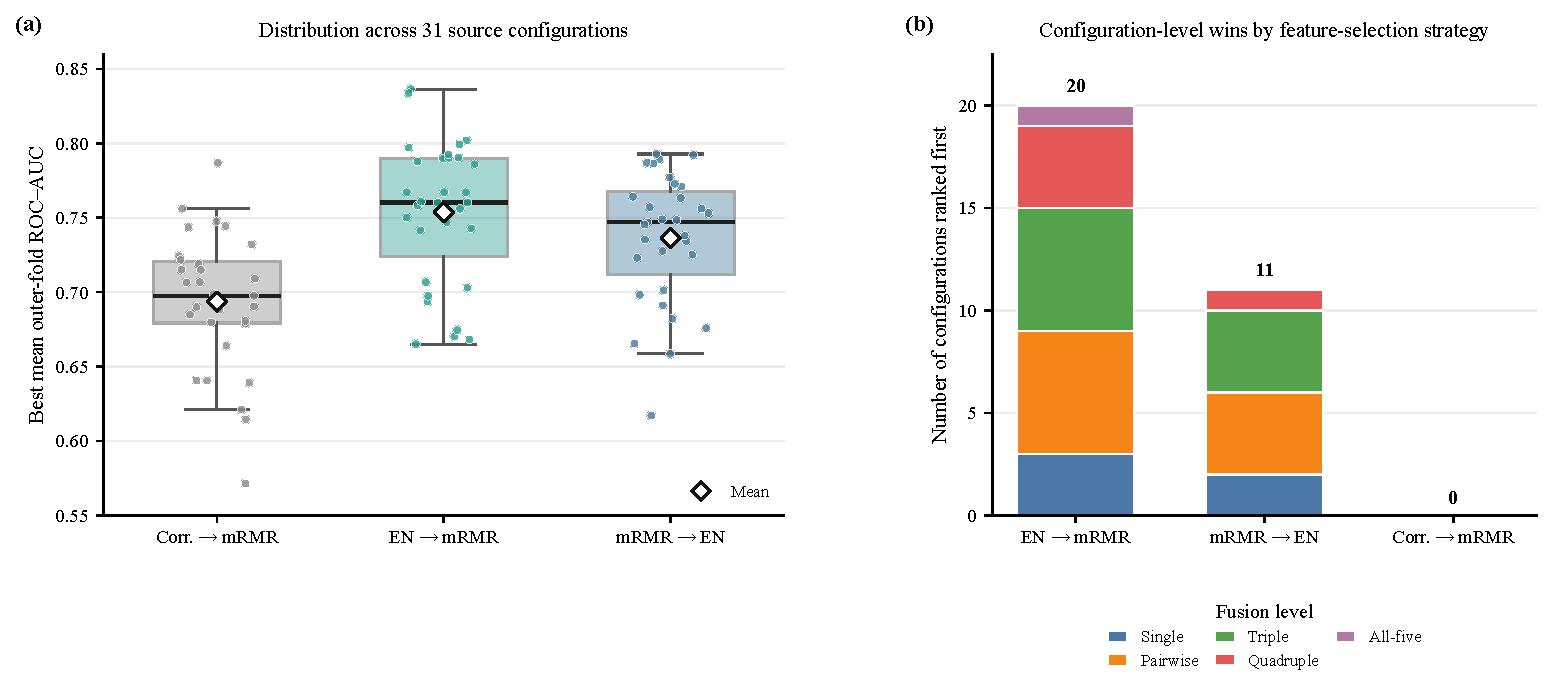
\includegraphics[width=\textwidth]
    {Figs/feature_selection_strategy_comparison.pdf}

    \caption{\textbf{Comparison of the three sequential
    feature-selection strategies across the 31 source configurations.}
    For each source configuration and feature-selection strategy, the
    displayed value represents the higher mean outer-fold ROC-AUC
    obtained after comparison of the SMOTE and no-SMOTE conditions
    and selection of the highest-performing classifier.
    (a) Distribution of the 31 method-specific mean outer-fold
    ROC-AUC values for each feature-selection strategy. Individual
    points represent source configurations, horizontal lines inside
    the boxes represent medians, boxes represent interquartile ranges,
    whiskers represent the remaining non-outlying range, and white
    diamond markers represent means.
    (b) Number of source configurations for which each strategy
    achieved the highest method-specific mean outer-fold ROC-AUC.
    Stacked bar segments indicate the contributions of single,
    pairwise, triple-source, quadruple-source, and complete
    five-source configurations. Numbers above the bars indicate the
    total number of configuration-level wins.
    EN, Elastic Net; mRMR, minimum redundancy maximum relevance.}
    \label{fig:feature_selection_comparison}
\end{figure*}

As shown in Figure~\ref{fig:feature_selection_comparison}(a), Elastic
Net followed by mRMR produced the highest average and median
method-specific mean outer-fold ROC-AUC. Its mean and median values
were 0.754 and 0.760, respectively. The corresponding values were
0.736 and 0.747 for mRMR followed by Elastic Net, and 0.694 and
0.698 for correlation filtering followed by mRMR.

The average mean ROC-AUC obtained with Elastic Net followed by mRMR
was approximately 0.018 higher than that obtained with mRMR followed
by Elastic Net and 0.060 higher than that obtained with correlation
filtering followed by mRMR.

Figure~\ref{fig:feature_selection_comparison}(b) shows that Elastic
Net followed by mRMR produced the highest method-specific mean
ROC-AUC in 20 of the 31 source configurations. mRMR followed by
Elastic Net ranked first in the remaining 11 configurations, whereas
correlation filtering followed by mRMR did not rank first in any
configuration.

At the single-source level, Elastic Net followed by mRMR ranked first
for three of the five datasets, whereas mRMR followed by Elastic Net
ranked first for two. The corresponding numbers were six and four
among the ten pairwise configurations, six and four among the ten
triple-source configurations, and four and one among the five
quadruple-source configurations. Elastic Net followed by mRMR also
produced the highest result for the complete five-source dataset.

The highest mean outer-fold ROC-AUC obtained using Elastic Net
followed by mRMR was 0.836 for ADC--Post1--Pre. The highest values
obtained using mRMR followed by Elastic Net and correlation filtering
followed by mRMR were 0.793 and 0.787, respectively.















\subsection{Effect of SMOTE on Classification Performance}
\label{subsec:smote_results}

The effect of SMOTE was evaluated separately for all 31 source
configurations. For each source configuration and SMOTE condition,
the pipeline with the highest mean outer-fold ROC-AUC was identified
after comparison of the three feature-selection strategies and ten
classifiers. This produced one best no-SMOTE result and one best
SMOTE result for each source configuration.

The SMOTE effect for source configuration \(d\) was calculated as

\[
\Delta\mathrm{AUC}_{d}
=
\mathrm{AUC}_{d,\mathrm{SMOTE}}
-
\mathrm{AUC}_{d,\mathrm{no\text{-}SMOTE}}.
\]

Positive values indicated higher mean outer-fold ROC-AUC with SMOTE,
whereas negative values indicated higher performance without SMOTE.
Figure~\ref{fig:smote_effect_comparison} shows the resulting
configuration-level differences and the number of wins obtained by
each balancing condition.




\begin{figure*}[htbp]
    \centering
    
\includegraphics[width=\textwidth]
    {Figs/smote_effect_across_31_configurations.pdf}


\caption{\textbf{Effect of SMOTE on classification performance across
the 31 source configurations.}
For each source configuration and balancing condition, the displayed
result corresponds to the pipeline with the highest mean ROC-AUC
after comparison of the three feature-selection strategies and ten
classifiers.
(a) Configuration-level difference in mean outer-fold ROC-AUC,
calculated as the best SMOTE result minus the best no-SMOTE result.
Dots represent individual source configurations, and horizontal stems
extend from zero to the corresponding difference. Positive values
indicate higher performance with SMOTE, whereas negative values
indicate higher performance without SMOTE. Configurations are grouped
according to feature-fusion level, and alternating background shading
separates these groups.
(b) Number of source configurations for which SMOTE or no-SMOTE
produced the higher mean outer-fold ROC-AUC at each feature-fusion
level. Numbers above individual bars indicate configuration-level
wins, and annotations above each pair indicate the total number of
configurations evaluated at that fusion level.}


    \label{fig:smote_effect_comparison}
\end{figure*}


As shown in Figure~\ref{fig:smote_effect_comparison}(a), most
configuration-level differences were located close to zero, although
both positive and negative effects were observed. The largest positive
difference was \(+0.025\) for Post1--Post2--Pre, whereas the largest
negative difference was \(-0.013\) for ADC--Post1--Pre.

Figure~\ref{fig:smote_effect_comparison}(b) shows that SMOTE produced
the higher mean outer-fold ROC-AUC in 19 of the 31 configurations,
compared with 12 configurations for no-SMOTE. The two conditions each
ranked higher in five pairwise and five triple-source configurations.
SMOTE ranked higher in all five quadruple-source configurations,
whereas no-SMOTE ranked higher for the complete five-source
configuration.


Across the 31 source configurations, the average of the best
no-SMOTE mean ROC-AUC values was 0.757, compared with 0.760 for the
best SMOTE results. The average configuration-level difference was
therefore \(+0.003\) in favour of SMOTE. The median difference was
also \(+0.003\).

SMOTE produced a higher best mean outer-fold ROC-AUC in 19 of the 31
source configurations, whereas no-SMOTE produced the higher result in
12 configurations. No exact ties were observed at the
configuration-level comparison.

The direction of the SMOTE effect differed among the feature-fusion
levels. SMOTE ranked higher for four of the five single-source
datasets, five of the ten pairwise configurations, five of the ten
triple-source configurations, and all five quadruple-source
configurations. The no-SMOTE condition ranked higher for the complete
five-source configuration.

The average SMOTE-minus-no-SMOTE difference was \(+0.010\) for the
single-source datasets, \(+0.0005\) for the pairwise configurations,
\(+0.0009\) for the triple-source configurations, and \(+0.006\) for
the quadruple-source configurations. The difference for the complete
five-source configuration was \(-0.005\).

For 26 of the 31 source configurations, the absolute difference
between the two balancing conditions was below 0.01 ROC-AUC. Four
configurations showed an improvement of at least 0.01 with SMOTE,
whereas one configuration showed a decrease of at least 0.01.

The largest positive difference was observed for
Post1--Post2--Pre. Its best mean outer-fold ROC-AUC increased from
0.728 without SMOTE to 0.753 with SMOTE, corresponding to a
difference of \(+0.025\). The largest negative difference occurred
for ADC--Post1--Pre, for which the best mean ROC-AUC decreased from
0.836 without SMOTE to 0.823 with SMOTE, corresponding to a
difference of \(-0.013\).

These results show that the direction and magnitude of the observed
SMOTE effect varied among source configurations. SMOTE was therefore
retained as an experimental pipeline condition rather than applied
uniformly to all datasets.








\subsection{Comparison of Machine-Learning Classifiers}
\label{subsec:classifier_results}

The classifiers represented in the highest-ranked pipelines were
examined across the 31 source configurations. For each source
configuration, one classifier was counted: the classifier belonging
to the pipeline with the highest mean outer-fold ROC-AUC after
comparison of the three feature-selection strategies and the two
SMOTE conditions.

Figure~\ref{fig:classifier_win_counts} summarises the number of
configuration-level selections obtained by each classifier and their
distribution across the five feature-fusion levels.



\begin{figure*}[htbp]
    \centering
    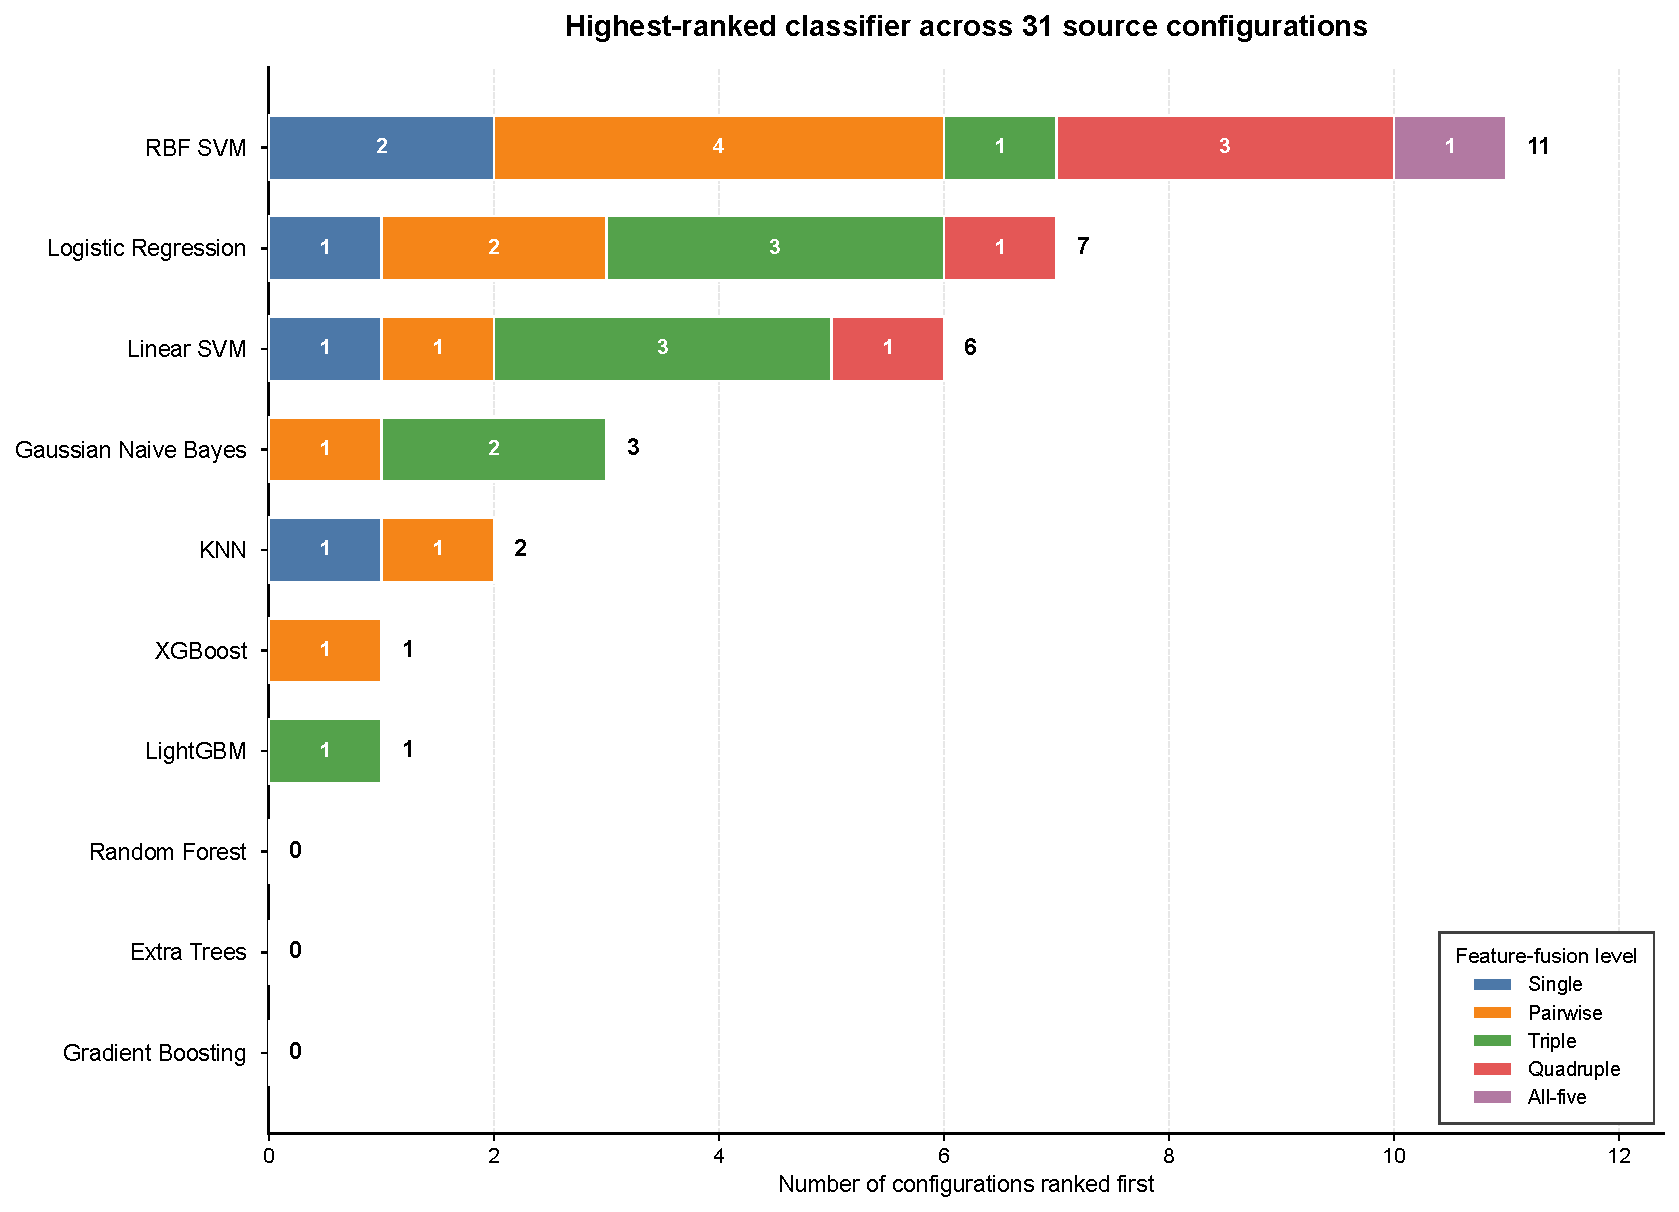
\includegraphics[width=0.92\textwidth]
    {Figs/classifier_win_counts_across_31_configurations.pdf}

    \caption{\textbf{Frequency of classifier selection among the
    highest-ranked pipelines across the 31 source configurations.}
    For each source configuration, the classifier belonging to the
    pipeline with the highest mean outer-fold ROC-AUC was counted
    after comparison of the three feature-selection strategies and
    the SMOTE and no-SMOTE conditions. Horizontal stacked bars show
    the numbers of configuration-level selections contributed by
    single-source, pairwise, triple-source, quadruple-source, and
    complete five-source analyses. Numbers within coloured segments
    indicate selections at the corresponding fusion level, whereas
    numbers at the ends of the bars indicate total selections across
    all fusion levels. Classifiers with no configuration-level
    selections are retained to show all ten models evaluated in the
    computational framework. KNN, K-Nearest Neighbours; SVM, support
    vector machine.}
    \label{fig:classifier_win_counts}
\end{figure*}



As shown in Figure~\ref{fig:classifier_win_counts}, RBF SVM was the
most frequently represented classifier among the highest-ranked
pipelines, with 11 configuration-level selections. Logistic
Regression and linear SVM followed with seven and six selections,
respectively. Together, the two SVM variants accounted for 17 of the
31 highest-ranked pipelines.

Gaussian Naive Bayes was selected in three configurations, and
K-Nearest Neighbours was selected in two. XGBoost and LightGBM were
each selected once. Random Forest, Extra Trees, and Gradient Boosting
did not appear in any configuration-level highest-ranked pipeline.



Seven of the ten candidate classifiers appeared in at least one
highest-ranked pipeline. RBF SVM was the most frequently selected
classifier, appearing in 11 of the 31 source configurations
(35.5\%). Logistic Regression ranked second, with seven selections
(22.6\%), followed by linear SVM with six selections (19.4\%).

The two SVM variants together accounted for 17 of the 31
highest-ranked pipelines. Gaussian Naive Bayes was selected in three
configurations, and K-Nearest Neighbours was selected in two.
XGBoost and LightGBM were each selected once.

Random Forest, Extra Trees, and Gradient Boosting did not appear in
the highest-ranked pipeline for any source configuration.

The distribution of classifier selections differed among the
feature-fusion levels. At the single-source level, RBF SVM was
selected for two datasets, while Logistic Regression, linear SVM, and
K-Nearest Neighbours were each selected once.

Among the ten pairwise configurations, RBF SVM was selected four
times, Logistic Regression twice, and linear SVM, Gaussian Naive
Bayes, K-Nearest Neighbours, and XGBoost once each.

At the triple-source level, Logistic Regression and linear SVM were
each selected for three configurations. Gaussian Naive Bayes was
selected twice, while RBF SVM and LightGBM were each selected once.

RBF SVM was selected for three of the five quadruple-source
configurations. Logistic Regression and linear SVM were each selected
once. RBF SVM was also the highest-ranked classifier for the complete
five-source configuration.

These frequencies describe how often each classifier appeared in a
configuration-level highest-ranked pipeline. They do not represent
the average performance of the classifier across all
feature-selection and SMOTE conditions.





\subsection{Detailed Performance of the Highest-Ranked Model}
\label{subsec:best_model_results}

The ADC--Post1--Pre configuration produced the highest mean
outer-fold ROC-AUC among the 31 evaluated source configurations. Its
highest-ranked pipeline combined Elastic Net followed by mRMR,
automatic feature-count selection, no SMOTE, and a linear SVM.

Figure~\ref{fig:best_model_oof_performance} presents the pooled
out-of-fold discrimination, threshold-dependent classification, and
probability-calibration results for this pipeline. All predictions
shown in the figure were generated for outer-test observations from
patients who were not included in the corresponding model-development
partition.

\begin{figure*}[htbp]
    \centering
    
\includegraphics[width=\textwidth]
    {Figs/best_overall_model_oof_performance.pdf}

    \caption{\textbf{Detailed out-of-fold performance of the
    highest-ranked machine-learning pipeline.}
    The selected pipeline combined the ADC, Post1, and Pre feature
    sources, Elastic Net followed by mRMR, automatic feature-count
    selection, no SMOTE, and a linear SVM. All panels were generated
    from pooled predictions for the five patient-aware outer-test
    folds.
    (a) Pooled receiver operating characteristic curve. The diagonal
    reference line represents chance-level discrimination.
    (b) Pooled precision--recall curve. The horizontal reference line
    represents the malignant-class prevalence of 0.558.
    (c) Pooled confusion matrix at the predefined malignant-class
    probability threshold of 0.5. Percentages are calculated relative
    to all 113 out-of-fold observations.
    (d) Pooled probability-calibration curve. The diagonal reference
    line represents perfect calibration.
    AUC, area under the curve; mRMR, minimum redundancy maximum
    relevance; SVM, support vector machine.}
    \label{fig:best_model_oof_performance}
\end{figure*}

The model achieved a mean outer-fold ROC-AUC of
\(0.836 \pm 0.088\). As shown in
Figure~\ref{fig:best_model_oof_performance}(a), combining the
predictions from the five outer-test folds produced a pooled ROC-AUC
of 0.799.

The mean outer-fold PR-AUC was 0.879, and the pooled out-of-fold
average precision was 0.832
(Figure~\ref{fig:best_model_oof_performance}(b)). The malignant-class
prevalence in the pooled out-of-fold dataset was 0.558.

At the predefined probability threshold of 0.5, the model correctly
classified 81 of the 113 ROIs, corresponding to a pooled accuracy of
0.717. The pooled confusion matrix contained 34 true-negative, 16
false-positive, 16 false-negative, and 47 true-positive predictions
(Figure~\ref{fig:best_model_oof_performance}(c)).

These classification counts corresponded to a sensitivity of 0.746,
specificity of 0.680, precision of 0.746, balanced accuracy of 0.713,
and F1-score of 0.746. The pooled Cohen's kappa was 0.426.

The pooled probability-calibration results are shown in
Figure~\ref{fig:best_model_oof_performance}(d). The corresponding
Brier score was 0.183.

Auto-\(k\) retained an average of 9.6 features across the five outer
folds. The selected feature count ranged from 4 to 18, with a median
of 8. Across the five folds, 28 distinct features appeared in at
least one selected subset. No feature was selected in all five folds,
and the most recurrent feature was selected in four folds. Detailed
feature-selection recurrence and model-interpretation results are
reported in Section~\ref{subsec:interpretability_results}.












\subsection{Feature-Selection Stability and Model Interpretation}
\label{subsec:interpretability_results}

Feature-selection stability and SHAP-based model interpretation were
examined for the highest-ranked ADC--Post1--Pre pipeline. This
pipeline combined Elastic Net followed by mRMR, automatic
feature-count selection, no SMOTE, and a linear SVM.

The feature-selection procedure was fitted independently within each
of the five patient-aware outer folds. Auto-\(k\) retained an average
of 9.6 features per outer-fold model, while 28 distinct features
appeared in at least one selected subset across the five folds. For
the stability analysis, a feature was considered recurrent when it
was selected in at least two of the five outer folds.

A total of 13 features satisfied this recurrence criterion
(Figure~\ref{fig:best_model_stability_shap}(a)). No feature was
selected in all five folds. The most recurrent feature was the ADC
intensity-histogram median
(\texttt{ADC\_IH\_IntensityHistogramMedian\_Intensity}), which was
selected in four of the five outer folds.

Five additional features were selected in three folds: the ADC
intensity-based median, the Post1 intensity-histogram minimum-gradient
grey-level feature, the Post1 intensity-histogram mode, Post1
Compactness~1, and the Post1 normalised zone-size non-uniformity
feature. The remaining seven recurrent features were selected in two
of the five folds. The recurrent feature set contained predictors
derived from ADC and Post1; no Pre-derived feature met the predefined
two-fold recurrence criterion.

\begin{figure*}[htbp]
    \centering
    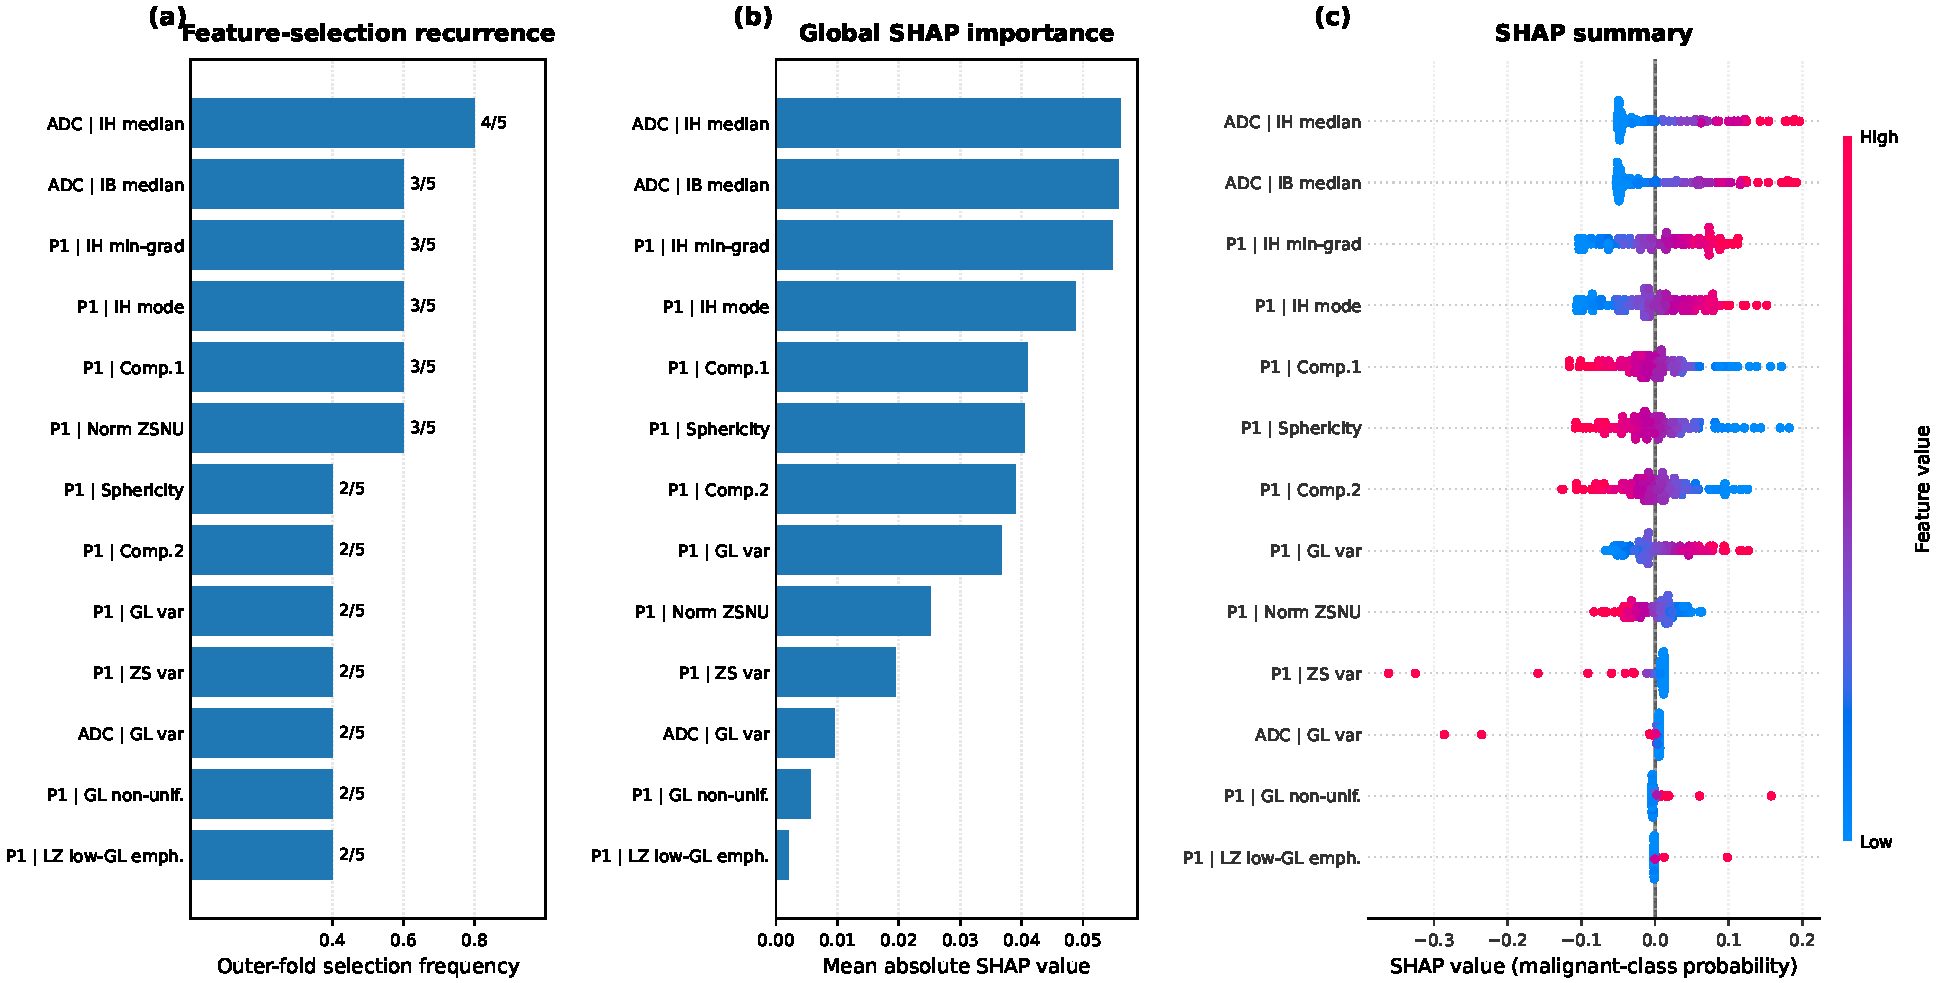
\includegraphics[width=\textwidth]
    {Figs/best_model_feature_stability_and_shap.pdf}

    \caption{\textbf{Feature-selection stability and SHAP
    interpretation of the highest-ranked ADC--Post1--Pre pipeline.}
    The selected pipeline combined Elastic Net followed by mRMR,
    automatic feature-count selection, no SMOTE, and a linear SVM.
    (a) Outer-fold recurrence of features selected in at least two of
    the five patient-aware outer folds. Bar lengths represent the
    proportion of outer folds in which each feature was retained, and
    labels indicate the corresponding selection count.
    (b) Global importance of the recurrent features in the
    full-cohort interpretation model, quantified using the mean
    absolute SHAP value.
    (c) SHAP summary plot showing feature contributions across
    individual ROIs. Horizontal position represents the SHAP value
    for the malignant-class probability, while colour represents the
    standardised feature value from low to high. Positive SHAP values
    increase the fitted model output toward the malignant class,
    whereas negative values decrease it. Feature names were shortened
    in the figure for readability.
    P1, Post1; IH, intensity histogram; IB, intensity based;
    Comp., compactness; GL, grey level; ZS, zone size; ZSNU,
    zone-size non-uniformity; LZ, large zone; mRMR, minimum
    redundancy maximum relevance; SHAP, Shapley Additive
    Explanations; SVM, support vector machine.
    The full-cohort refit was used for interpretation only; all
    predictive-performance estimates reported in this study were
    obtained from patient-aware out-of-fold predictions.}
    \label{fig:best_model_stability_shap}
\end{figure*}

For model interpretation, a separate linear SVM was refitted using
the recurrent feature set and the complete cohort. This refit was
performed only to obtain a single model for SHAP analysis and was
not used to estimate predictive performance. All reported
classification-performance measures remained based on the nested
cross-validation out-of-fold predictions.

As shown in Figure~\ref{fig:best_model_stability_shap}(b), the ADC
intensity-histogram median and ADC intensity-based median had the
largest mean absolute SHAP values among the recurrent features. The
Post1 intensity-histogram minimum-gradient grey-level feature and
Post1 intensity-histogram mode followed them in the global importance
ranking. Several Post1 morphological and grey-level size-zone matrix
features also contributed to the interpretation model.

The SHAP summary plot
(Figure~\ref{fig:best_model_stability_shap}(c)) additionally shows the
direction and observation-level variability of these contributions.
Higher standardised values of the two leading ADC intensity features
were generally associated with positive SHAP values, corresponding
to a higher fitted malignant-class probability. Higher values of the
two leading Post1 intensity-histogram features were also predominantly
associated with positive contributions.

In contrast, higher values of several Post1 morphological features,
including Compactness and Sphericity, were more frequently associated
with negative SHAP contributions. Other recurrent features showed
smaller or more heterogeneous contributions across individual ROIs.

Feature-selection recurrence and SHAP importance represented
different properties of the modelling pipeline. Selection frequency
described how consistently a predictor was retained when the training
patients changed, whereas mean absolute SHAP value described its
average contribution within the fitted interpretation model.
Accordingly, a feature with relatively high recurrence did not
necessarily have the highest SHAP importance, and vice versa. SHAP
values were interpreted as explanations of the fitted model rather
than as evidence of causal or biological relationships.







\section{Discussion}
\label{sec:discussion}

\subsection{Principal Findings}
\label{subsec:discussion_principal_findings}

This study systematically evaluated single- and multi-source radiomic
feature representations within a patient-aware machine-learning
framework. All 31 non-empty combinations of five MRI-derived feature
sources were examined using the same nested cross-validation design,
three sequential feature-selection strategies, optional SMOTE, and
ten machine-learning classifiers. The main finding was that the
highest classification performance was obtained from a selected
triple-source representation rather than from complete concatenation
of all available feature sources.

The highest-ranked pipeline combined ADC, Post1, and Pre features with
Elastic Net followed by mRMR, automatic feature-count selection, no
SMOTE, and a linear SVM. It achieved a mean outer-fold ROC-AUC of
\(0.836 \pm 0.088\). A second triple-source configuration,
ADC--Post2--T2, achieved a very similar mean ROC-AUC of
\(0.834 \pm 0.045\). In contrast, the complete five-source
configuration achieved a lower mean ROC-AUC of
\(0.747 \pm 0.117\). These results indicate that increasing the number
of concatenated feature sources did not produce a monotonic
improvement in classification performance.

The comparison of feature-selection strategies further showed that
the order in which dimensionality-reduction methods were applied was
relevant to model performance. Elastic Net followed by mRMR produced
the highest configuration-level result in 20 of the 31 source
configurations and also showed the highest average method-specific
mean ROC-AUC. mRMR followed by Elastic Net ranked first in the
remaining 11 configurations, whereas correlation filtering followed
by mRMR did not produce the highest result for any configuration.

The effect of SMOTE was comparatively small and varied among source
configurations. Although SMOTE produced the higher configuration-level
result more often than the no-SMOTE condition, most differences in
mean outer-fold ROC-AUC were close to zero. The highest-ranked model
in the complete study was obtained without SMOTE. This finding
supports evaluating synthetic oversampling as a model-development
choice rather than assuming that it will consistently improve
classification performance when class imbalance is limited.

Classifier selection also varied across source configurations. RBF
SVM was the most frequently represented classifier among the
highest-ranked pipelines, followed by Logistic Regression and linear
SVM. Nevertheless, the best overall model used a linear SVM. Thus,
the classifier that was selected most frequently across datasets was
not necessarily the classifier associated with the single highest
ROC-AUC.

The detailed analysis of the highest-ranked ADC--Post1--Pre model
showed a pooled out-of-fold ROC-AUC of 0.799 and a pooled PR-AUC of
0.832. At the predefined probability threshold of 0.5, the model
produced a balanced accuracy of 0.713 and an F1-score of 0.746.
These pooled results were lower than the mean outer-fold ROC-AUC,
illustrating that fold-averaged and pooled measures provide related
but non-equivalent summaries of predictive performance.

Feature-selection analysis additionally showed that the final models
were compact relative to the original feature space but that the
identity of the retained features varied across patient groups. The
highest-ranked model selected an average of 9.6 features per outer
fold, while 28 distinct features appeared across the five folds. Only
13 features were selected in at least two folds, and none was selected
in every fold. This variability indicates that similar predictive
performance could be obtained from partially different feature subsets
when the model was trained on different groups of patients.

The SHAP analysis of the recurrent feature set showed that the fitted
interpretation model relied most strongly on two ADC-derived intensity
features, followed by several Post1 intensity, morphological, and
grey-level size-zone matrix features. These interpretation results
were considered complementary to the stability analysis: selection
frequency described how consistently a feature was retained across
training subsets, whereas SHAP values described how strongly the
refitted model used that feature once included.

Taken together, the findings support three main observations. First,
selective multi-source feature integration performed better than
complete feature concatenation in this dataset. Second, feature
selection and classifier choice interacted with the source
representation, such that no single modelling component was uniformly
optimal across all configurations. Third, patient-aware validation
revealed substantial variation in both predictive performance and
selected feature identity across patient subsets, highlighting the
importance of evaluating not only peak model performance but also the
stability of the complete modelling procedure.










\subsection{Effect of Multi-Source Feature Integration}
\label{subsec:discussion_feature_integration}

A central objective of this study was to determine whether combining
radiomic feature sources improved classification performance relative
to analysing the individual sources separately. The results showed
that multi-source integration could improve performance, but that the
improvement depended strongly on which sources were combined. The
relationship between the number of concatenated sources and
classification performance was therefore not monotonic.

The best single-source configuration achieved a mean outer-fold
ROC-AUC of 0.790, which increased to 0.799 for the highest-ranked
pairwise configuration and to 0.836 for the highest-ranked
triple-source configuration. Performance did not continue to increase
when additional sources were included. The best quadruple-source
configuration achieved a mean ROC-AUC of 0.802, while complete
five-source concatenation produced a lower value of 0.747. Thus, the
highest performance was obtained from a selected subset of three
sources rather than from the complete available feature set.

One possible explanation is the rapid increase in dimensionality
created by feature concatenation. The single-source datasets contained
approximately 145 candidate predictors, whereas the triple-source
datasets contained approximately 435 predictors, the quadruple-source
datasets approximately 580, and the complete five-source dataset 724.
In contrast, the number of patients remained fixed at approximately
48, and the number of matched ROIs remained close to 113--117.
Consequently, adding a feature source increased the number of
candidate variables without providing a corresponding increase in the
number of independent training patients.

This increasing predictor-to-patient ratio can make model development
more difficult. When the candidate feature space becomes larger, the
feature-selection procedure must identify a small informative subset
from a progressively larger number of alternatives. Additional
variables may provide useful complementary information, but they may
also introduce redundant or weakly informative predictors. In a
limited cohort, distinguishing reliably between these possibilities
can become increasingly sensitive to the particular patients included
in the training partition.

The Auto-\(k\) procedure partially controlled this increase in
dimensionality by restricting the final classifier to a relatively
small feature subset. For example, the highest-ranked
ADC--Post1--Pre model retained an average of only 9.6 features per
outer fold despite starting from more than 400 candidate predictors.
Nevertheless, feature selection must still operate on the larger
initial search space before this compact representation is obtained.
The observed reduction in performance with complete feature
concatenation therefore cannot be interpreted simply as a consequence
of the final number of variables supplied to the classifier.

The configuration-level results also indicate that the identity of the
combined sources was more important than the number of sources alone.
Several triple-source combinations performed substantially better than
other triple-source combinations, despite having almost identical
numbers of observations and predictor variables. Similarly, the ten
pairwise configurations covered a broad range of mean ROC-AUC values.
This variation suggests that feature-fusion level by itself provides
an incomplete description of model performance.

ADC was present in the highest-ranked pairwise, triple-source, and
quadruple-source configurations, and the highest-performing
triple-source configurations also contained ADC. However, the present
analysis does not establish that ADC is independently responsible for
the observed improvements. The contribution of one source depends on
the other sources with which it is combined, the features retained in
each training fold, and the classifier selected for the corresponding
pipeline.

The lower performance of the complete five-source model should
therefore not be interpreted as evidence that one or more individual
sources are inherently uninformative. A source that does not improve
performance when concatenated with all other sources may still
contribute useful predictors in a smaller combination. Conversely,
adding an individually useful source to an already informative feature
representation may provide little additional predictive information
while increasing the dimensionality of the candidate space.

These findings support evaluating source combinations explicitly
rather than assuming that complete feature concatenation is the
preferred multi-source strategy. In datasets with a limited number of
independent patients, selective feature-source integration can provide
a more effective representation than combining every available source.
External validation in a larger cohort will be required to determine
whether the relative advantage of the selected triple-source
configuration is reproducible.












\subsection{Influence of Feature-Selection Strategy}
\label{subsec:discussion_feature_selection}

Feature-selection strategy had a clear influence on the performance
of the evaluated pipelines. Elastic Net followed by mRMR produced the
highest configuration-level result in 20 of the 31 source
configurations and had the highest average method-specific mean
outer-fold ROC-AUC. mRMR followed by Elastic Net ranked first in the
remaining 11 configurations, whereas correlation filtering followed
by mRMR did not produce the highest-ranked result for any source
configuration.

These findings indicate that the order of sequential feature-selection
operations was relevant. Elastic Net followed by mRMR and mRMR
followed by Elastic Net contained the same two component methods, but
they operated on different intermediate feature spaces. The first
stage determined which predictors remained available to the second
stage and could therefore change the final subset even when the same
target feature count was requested.

In the Elastic-Net--mRMR pipeline, Elastic Net first performed a
supervised and regularised reduction of the full candidate feature
space. The resulting candidate pool was then processed by mRMR, which
favoured features with high relevance to the target while penalising
redundancy with features that had already been selected. One possible
advantage of this ordering is that the second-stage mRMR procedure
operated on a smaller candidate space that had already undergone
supervised regularised screening.

The reverse pipeline began by applying mRMR directly to the complete
feature space and then used Elastic Net to rank the reduced candidate
pool. This strategy remained competitive and produced the
highest-ranked result in approximately one third of the source
configurations. Its performance therefore shows that there was no
universally optimal ordering of the two selectors. Nevertheless, the
more frequent wins and higher average ROC-AUC observed for
Elastic Net followed by mRMR suggest that this ordering was better
suited to the present datasets.

Correlation filtering followed by mRMR showed lower performance than
the two Elastic-Net-based strategies. The correlation stage removed
features when their absolute pairwise Pearson correlation exceeded
0.90 and retained one representative using direction-independent
univariate ROC-AUC. This procedure can efficiently reduce strongly
redundant predictors, but it considers pairwise linear correlation
before the subsequent multivariable selection stage. In a
high-dimensional radiomic feature space, correlated predictors may
not be interchangeable with respect to their contribution in
combination with other variables. Consequently, an early correlation
filter may remove predictors that would otherwise contribute useful
information to a multivariable model.

This interpretation should remain cautious. The present experiments
did not isolate the individual causal contribution of each
feature-selection operation, and the three strategies were compared
within the same finite cohort. Their relative ordering may therefore
depend on the specific feature distributions, patient composition,
candidate feature counts, and cross-validation partitions used in
this study.

The results also show that feature-selection performance should not be
judged only by the single highest ROC-AUC obtained in the study.
Although Elastic Net followed by mRMR produced the overall
highest-ranked model, mRMR followed by Elastic Net remained preferable
for 11 source configurations. This variation reinforces the need to
treat feature selection as part of the complete modelling pipeline
rather than as a fixed preprocessing operation that can be selected
independently of the input representation.

Overall, the results support the use of sequential supervised feature
selection for these high-dimensional datasets, with Elastic Net
followed by mRMR providing the most consistently favourable results
among the three evaluated strategies. Confirmation in an independent
cohort would be required before considering this ordering generally
preferable for radiomic classification tasks.











\subsection{Effect of SMOTE and Class Imbalance}
\label{subsec:discussion_smote}

SMOTE did not produce a uniform improvement in classification
performance. At the source-configuration level, the best SMOTE
pipeline achieved a higher mean outer-fold ROC-AUC in 19 of the 31
configurations, whereas the best no-SMOTE pipeline ranked higher in
12. However, the magnitude of most differences was small. Therefore,
the larger number of SMOTE wins should not be interpreted as evidence
of a substantial general improvement in discrimination.

This distinction between win frequency and effect size is important.
A source configuration was counted as a SMOTE win even when the
difference in mean ROC-AUC was only a few thousandths. Consequently,
a larger number of configuration-level wins can coexist with an
average ROC-AUC difference close to zero. In the present experiments,
the largest positive configuration-level difference was only 0.025,
while the largest negative difference was 0.013.

The limited overall effect of SMOTE is also consistent with the class
distribution of the datasets. The imbalance between benign and
malignant ROIs was relatively modest. For example, the complete
five-source dataset contained 50 benign and 63 malignant ROIs.
Synthetic oversampling therefore modified a dataset that was not
severely imbalanced. Under these conditions, the additional synthetic
observations may alter the fitted decision boundary without producing
a substantial improvement in the overall ranking of unseen
observations.

An important distinction is that ROC-AUC is threshold independent,
whereas several other classification measures depend on the selected
decision threshold. SMOTE changes the training distribution and can
therefore alter classifier coefficients, support vectors,
neighbourhood relationships, or tree structures. These changes may
affect sensitivity and specificity at a fixed threshold even when the
relative ranking of observations, and therefore ROC-AUC, changes only
slightly.

The more detailed paired analyses performed in this study were
consistent with this interpretation. Across dataset and
feature-selection comparisons, SMOTE had almost no average effect on
mean outer-fold ROC-AUC but tended to increase pooled balanced
accuracy. This improvement was accompanied by a shift in
class-specific performance: specificity generally increased, whereas
sensitivity tended to decrease. Because the positive class in this
study represented malignant ROIs, this pattern corresponds to improved
recognition of the smaller benign class at the cost of some reduction
in malignant-class sensitivity.

This trade-off also explains why the effect of SMOTE depended on the
performance measure considered. A model may achieve higher balanced
accuracy or specificity while showing little change in ROC-AUC, and
an improvement in precision may occur together with a reduction in
sensitivity. SMOTE should therefore not be judged using only whether
it increases one threshold-dependent metric.

The effect of oversampling also varied with feature-selection strategy
and source configuration. This is expected because SMOTE generates
synthetic observations by interpolation in the selected feature
space. The geometry of that space changes when different predictors
are retained, and the same synthetic-sampling procedure may therefore
modify different classifiers in different ways. For example,
synthetic samples can directly change local neighbourhoods for KNN,
the position of support vectors for SVMs, and candidate partitions for
tree-based models.

Importantly, the two highest-ranked triple-source configurations,
ADC--Post1--Pre and ADC--Post2--T2, were both obtained without
SMOTE. The complete five-source winner was also a no-SMOTE pipeline.
These findings show that synthetic oversampling was not required to
achieve the strongest discrimination observed in the study.

Conversely, SMOTE was selected in several successful pipelines,
including all five configuration-level winners in the
quadruple-source analysis. Its usefulness was therefore
configuration-dependent rather than uniformly absent. The results do
not support removing SMOTE from consideration; instead, they support
evaluating it within the model-development procedure and retaining it
only when it improves the predefined optimisation objective.

SMOTE and decision-threshold adjustment should also be regarded as
different operations. SMOTE changes the training data before model
fitting and can alter the fitted decision function itself. Threshold
adjustment does not refit the model and instead changes only the point
at which a continuous model output is converted into a class label.
If the primary objective is to change the sensitivity--specificity
trade-off rather than improve ranking performance, threshold
optimisation may therefore represent a distinct and potentially more
direct strategy.

In the present study, mean outer-fold ROC-AUC was predefined as the
primary model-ranking measure. According to this criterion, SMOTE
provided no consistent or substantial general advantage. Its effects
on balanced accuracy and class-specific error rates remain relevant,
but these complementary changes should be considered in relation to
the intended application rather than interpreted as evidence that
synthetic oversampling is universally beneficial.









\subsection{Classifier Performance and Model Complexity}
\label{subsec:discussion_classifiers}

Classifier performance varied across source configurations, and no
single classifier was optimal for every dataset. Nevertheless, the
highest-ranked pipelines were concentrated among a relatively small
subset of the ten evaluated models. RBF SVM was the most frequently
selected classifier, appearing in 11 of the 31 configuration-level
winners, followed by Logistic Regression in seven configurations and
linear SVM in six. Together, the two SVM variants accounted for 17
of the 31 highest-ranked pipelines.

The frequent selection of SVM-based models is compatible with the
structure of the present classification problem. After feature
selection, each outer-fold classifier was fitted using a relatively
small number of predictors but a limited number of independent
patients. Margin-based classifiers can provide flexible decision
boundaries while controlling model complexity through regularisation.
The linear and RBF variants also allowed the analysis to test whether
the selected feature representation was more appropriately separated
by a linear or nonlinear boundary.

The overall highest-ranked model used a linear SVM rather than the
more frequently selected RBF SVM. This finding is important because
classifier win frequency and peak predictive performance measure
different properties. RBF SVM was selected most often across the 31
source configurations, but the highest individual mean outer-fold
ROC-AUC was obtained using a linear decision boundary for the
ADC--Post1--Pre representation.

A linear classifier performing well after feature selection may
indicate that the retained variables provide a representation in which
substantial class separation can be captured without a highly complex
decision function. However, this should not be interpreted as evidence
that the underlying relationships among all original radiomic features
are strictly linear. The feature-selection stages were supervised and
could remove variables that were less useful for the final
classification problem, thereby changing the geometry of the input
space presented to the classifier.

Logistic Regression was also frequently represented among the
highest-ranked pipelines. Both Logistic Regression and linear SVM
apply regularised linear decision functions, although they optimise
different objectives and produce different probability estimates.
Their frequent selection suggests that comparatively simple
regularised models remained competitive after dimensionality
reduction.

In contrast, the tree-based ensemble models were less frequently
represented among the configuration-level winners. XGBoost and
LightGBM were each selected once, while Random Forest, Extra Trees,
and Gradient Boosting did not appear in any final
configuration-level winning pipeline. This result does not establish
that tree-based methods are generally unsuitable for radiomic
classification. Rather, within the present dataset size, selected
feature representations, hyperparameter search spaces, and nested
cross-validation procedure, they did not achieve the highest mean
outer-fold ROC-AUC for the evaluated source configurations.

One possible explanation is that flexible ensemble models require
sufficient training data to estimate complex interactions reliably.
In the present study, the number of independent patients was small
relative to the original number of candidate predictors. Although
feature selection substantially reduced the dimensionality before
classifier fitting, the effective training sample in each outer and
inner fold remained limited. Under such conditions, additional model
flexibility may not necessarily translate into improved performance
on previously unseen patients.

The restricted hyperparameter-optimisation budget should also be
considered when interpreting classifier comparisons. Each Optuna
study evaluated ten candidate hyperparameter configurations. This
provided a consistent computational budget across classifiers but was
not intended to exhaustively explore every possible region of the
search space. Models with larger or more complex hyperparameter
spaces, particularly boosted-tree methods, may therefore have been
more sensitive to the limited tuning budget than models with only one
or two principal hyperparameters.

K-Nearest Neighbours and Gaussian Naive Bayes occasionally produced
the highest-ranked result for individual source configurations,
showing that comparatively simple non-linear or probabilistic
approaches could also be competitive for particular feature
representations. Their limited number of wins, however, indicates
that their performance was more configuration specific.

The classifier results therefore reinforce the importance of
evaluating the classifier together with the preceding feature
representation rather than treating model choice as an isolated
decision. The optimal classifier depended on the source combination,
selected feature subset, and class-balancing condition. In the present
study, regularised linear and kernel-based models provided the most
frequent high-performing solutions, while the single best-performing
pipeline used the simpler linear SVM.














\subsection{Feature Stability and Model Interpretation}
\label{subsec:discussion_interpretability}

The feature-stability analysis provided information that was not
captured by predictive-performance measures alone. Although the
highest-ranked ADC--Post1--Pre pipeline retained an average of only
9.6 features in each outer-fold model, the identity of these features
varied when the training patients changed. Across the five outer
folds, 28 distinct features were selected at least once, while only
13 were retained in two or more folds and no feature was selected in
all five folds.

This finding highlights an important distinction between model
performance and feature-selection stability. A pipeline can maintain
relatively strong classification performance while selecting
partially different subsets of correlated or similarly informative
predictors in different training samples. In high-dimensional
radiomic datasets, several features may contain overlapping
information, allowing different subsets to support similar predictive
functions.

The limited recurrence observed in the present study may also reflect
the small number of independent patients relative to the original
feature space. Each change in the outer-training population alters
the data available to the supervised feature-selection procedure.
With hundreds of candidate predictors and a comparatively small
training cohort, modest changes in the training observations can
change feature rankings and therefore the subset passed to the final
classifier.

Sequential feature selection may further contribute to this
variability. In the highest-ranked pipeline, Elastic Net first
reduced the candidate space and mRMR subsequently selected a compact
subset from the retained predictors. A feature excluded during the
first stage was no longer available to the second stage, and small
changes in Elastic-Net coefficients across training folds could
therefore propagate to the final selected subset. Similarly, the
mRMR redundancy term depends on features that have already been
selected and can lead to different choices among correlated
candidates.

The stability results therefore suggest that individual selected
features should be interpreted more cautiously than the predictive
performance of the complete pipeline. A feature that appeared in only
one outer fold may still have contributed to a valid predictive model
in that fold, but its limited recurrence provides weaker evidence that
it represents a robust predictor across patient subsets. Conversely,
features selected repeatedly across several folds provide stronger
evidence of selection stability, although recurrence alone does not
measure their contribution to the classifier output.

This distinction was apparent when feature-selection frequency was
compared with SHAP importance. The most recurrent ADC
intensity-histogram median feature also had the largest mean absolute
SHAP value in the interpretation model, but recurrence and SHAP
importance were not identical rankings for all features. Selection
frequency measures how consistently a variable survives the
model-development procedure, whereas SHAP measures its contribution
after the variable has been included in a fitted model.

The recurrent feature set for the highest-ranked pipeline contained
features derived from ADC and Post1. No Pre-derived feature satisfied
the predefined requirement of selection in at least two outer folds.
This observation should not be interpreted as showing that the Pre
source was uninformative. The highest-performing source
configuration itself included Pre, and different Pre-derived features
could have contributed in individual folds without recurring often
enough to enter the stability-based interpretation set. In addition,
the contribution of one source may be expressed through interactions
or through changes in which features from the other sources are
selected.

The SHAP analysis indicated that the full-cohort interpretation model
relied most strongly on two ADC-derived intensity features, followed
by several Post1 intensity, morphological, and grey-level size-zone
matrix features. Higher values of the leading ADC intensity features
were generally associated with positive SHAP contributions in the
fitted model, whereas several Post1 morphological features showed the
opposite tendency. These directions describe how the fitted classifier
used the standardised predictors and should not be interpreted as
direct biological or causal effects.

An additional limitation is that SHAP values were calculated from a
separate model refitted using the complete cohort and the recurrent
feature set. This refit was necessary to provide one common model for
interpretation, but its predictions were not used to estimate
classification performance. The reported ROC-AUC, PR-AUC, and
threshold-dependent metrics remained based on patient-aware
out-of-fold predictions. Consequently, the SHAP analysis should be
viewed as an explanation of the final fitted representation rather
than as an independent validation of feature importance.

Overall, the stability and interpretation analyses support reporting
the selected predictors as a recurrent feature set rather than as a
single fixed signature. The observed variability indicates that
external validation should assess not only whether predictive
performance is reproduced, but also whether the same feature sources,
feature families, and individual predictors continue to be selected
in an independent cohort.











\subsection{Strengths and Limitations}
\label{subsec:discussion_strengths_limitations}

Several aspects of the computational design strengthen the reliability
of the present analysis. First, model evaluation was patient aware.
Although individual ROIs were used as prediction units, all ROIs from
the same patient were assigned to the same cross-validation partition.
This prevented observations from the same patient from appearing
simultaneously in training and test data and reduced the risk of
patient-level information leakage.

Second, model development was performed within a nested
cross-validation framework. Hyperparameter optimisation, feature
selection, feature-count selection, preprocessing, and the optional
application of SMOTE were restricted to the training data available
within the corresponding cross-validation stage. The outer folds were
therefore not used to fit these components before prediction. This
design provides a more realistic estimate of performance on unseen
patients than procedures in which feature selection or
hyperparameter optimisation is performed before cross-validation.

Third, the study evaluated the complete set of 31 non-empty
combinations of the five available radiomic feature sources using a
common computational framework. The same three feature-selection
strategies, SMOTE comparison, classifier set, optimisation procedure,
and primary evaluation criterion were applied across the source
configurations. This systematic design allowed differences among
single- and multi-source representations to be evaluated under
largely consistent modelling conditions rather than by comparing
independently developed pipelines.

The analysis also extended beyond a single discrimination metric.
Mean outer-fold ROC-AUC was predefined as the primary model-ranking
criterion, while pooled out-of-fold ROC-AUC, PR-AUC,
threshold-dependent classification metrics, calibration, feature
recurrence, and SHAP-based interpretation provided complementary
information. In particular, the stability analysis showed that a
high-performing model can remain predictive while selecting partially
different feature subsets across training samples, which would not
have been apparent from ROC-AUC alone.

These strengths should be considered together with several important
limitations. The principal limitation is the small number of
independent patients. The datasets contained approximately 48
patients, despite including more than 100 ROIs. Because
cross-validation was grouped at the patient level, the effective
number of independent units available for model development remained
limited. This is particularly important for the multi-source datasets,
in which several hundred candidate predictors were available before
feature selection.

The use of multiple ROIs per patient also means that the reported
classification results are ROI-level rather than patient-level
performance estimates. Patient grouping prevents leakage across
cross-validation folds, but it does not convert multiple observations
from one patient into independent patients. Consequently, the number
of ROIs should not be interpreted as the effective sample size of the
study.

A further limitation is the absence of an independent external test
cohort. Nested cross-validation reduces optimisation bias within each
model-development procedure, but all source configurations and
modelling strategies were ultimately compared using the same study
cohort. The highest-ranked pipeline was selected from a large number
of evaluated alternatives, and its observed performance may therefore
include some degree of selection optimism. External validation is
required to determine whether the ranking of source configurations
and the performance of the ADC--Post1--Pre pipeline are reproducible
in independent data.

The computational search was also necessarily constrained. Ten
classifiers, three feature-selection strategies, two SMOTE
conditions, multiple candidate feature counts, and 31 source
configurations already produced a large model-development space.
Optuna was therefore limited to ten trials for each optimisation
study. This ensured a consistent and computationally manageable
search procedure, but it should not be interpreted as exhaustive
hyperparameter optimisation. Classifiers with larger or more complex
hyperparameter spaces may have benefited from a larger optimisation
budget.

The study used direct feature concatenation to construct multi-source
datasets. This approach provides a transparent way to compare all
source combinations, but it does not explicitly model relationships
between sources. Alternative integration methods, including
source-specific dimensionality reduction, late fusion, representation
learning, or other multimodal modelling strategies, could produce
different results and were outside the scope of the present analysis.

Feature-selection stability represents another limitation. The
highest-ranked model retained a compact number of predictors in each
outer fold, but the selected feature identities varied across folds,
and no individual feature was selected in all five folds. The SHAP
results should therefore be interpreted as descriptions of the fitted
model rather than evidence of a fixed or externally validated feature
signature.

In addition, the SHAP analysis required a separate full-cohort refit
using the recurrent feature set to obtain one common model for
interpretation. This model was used only to explain fitted prediction
behaviour and not to estimate predictive performance. Nevertheless,
its SHAP values describe a model fitted to the complete available
cohort and therefore do not constitute independent evidence that the
same feature contributions will be reproduced in new patients.

Calibration and threshold-dependent metrics should also be interpreted
cautiously. The limited cohort size restricts the number of
observations available within calibration bins, and the fixed
probability threshold of 0.5 was not optimised for a particular
clinical operating point. Sensitivity, specificity, precision, and
related measures could therefore change if a different decision
threshold were selected in an independent development cohort.

Finally, the present work was designed as a computational evaluation
of radiomic machine-learning strategies. It does not establish causal
or biological interpretations of individual radiomic features, nor
does it demonstrate clinical utility. The reported results should
therefore be considered evidence regarding the comparative behaviour
of the evaluated modelling pipelines within the available cohort,
rather than confirmation of a deployable diagnostic model.

Despite these limitations, the combination of patient-aware nested
cross-validation, training-only preprocessing, systematic comparison
of source combinations, and out-of-fold performance evaluation
provides a controlled framework for identifying candidate modelling
strategies for subsequent independent validation.









\subsection{Future Work and Generalisability}
\label{subsec:discussion_future_work}

The next priority is independent validation of the highest-ranked
ADC--Post1--Pre pipeline. Although patient-aware nested
cross-validation was used throughout the present study, all model
development and configuration comparisons were performed within a
single cohort. Evaluation in an independent dataset is therefore
required to determine whether the observed discrimination and the
relative advantage of the selected triple-source representation are
reproducible.

External validation should preserve the patient-level grouping used in
the present analysis and should evaluate the complete modelling
pipeline rather than only the final classifier. This includes the
preprocessing operations, feature-selection sequence, automatic
feature-count selection, and classifier specification. Reapplying
feature selection within the external development process will also be
important for determining whether the recurrent features identified
in the present cohort remain stable when the patient population
changes.

A larger cohort would additionally allow more precise estimation of
predictive performance. In the present study, the limited number of
independent patients contributed to variability across outer folds and
restricted the precision of calibration and threshold-dependent
performance estimates. Increasing the number of patients, rather than
only the number of ROIs, would provide a stronger basis for estimating
generalisation performance and feature-selection stability.

Future studies should also investigate whether the relative advantage
of selective source integration persists in larger datasets. The
present results favoured specific triple-source combinations over
complete five-source concatenation, but this relationship may change
as the number of training patients increases. A larger cohort may
allow models to make more effective use of additional predictors and
may reduce the instability associated with selecting a small feature
subset from a very high-dimensional candidate space.

The present multi-source analysis used direct feature concatenation,
which was intentionally chosen for transparency and systematic
comparison of all 31 source combinations. Future computational work
could compare this strategy with alternative fusion methods. Examples
include source-specific feature selection followed by late fusion,
separate source-level classifiers with prediction-level combination,
or representation-learning approaches designed to preserve
source-specific information before integration. Such comparisons
would help determine whether the lower performance observed with
complete concatenation resulted from the information content of the
sources themselves or from the way in which the feature spaces were
combined.

More extensive hyperparameter optimisation may also be useful,
particularly for classifiers with relatively large search spaces.
The present ten-trial Optuna budget provided a consistent search
procedure across a large number of pipelines, but it was not intended
to identify the global optimum for every classifier. A future
validation study could allocate a larger optimisation budget to a
smaller set of candidate pipelines identified from the current
screening analysis.

Model calibration and decision-threshold selection represent further
areas for investigation. The present study used a fixed probability
threshold of 0.5 for threshold-dependent metrics and did not optimise
a threshold for a specific operating objective. In future work,
threshold selection could be performed exclusively within training
data and then evaluated on independent patients. This would allow
sensitivity, specificity, precision, and related measures to be
adapted to a predefined application requirement without introducing
test-set optimisation.

The feature-stability analysis should also be repeated in independent
data. Reproducibility of individual feature names would provide the
strongest evidence of a stable signature, but stability can also be
examined at broader levels, including feature source and feature
family. This distinction may be useful when several correlated
radiomic variables represent similar information and individual
feature identities vary across samples.

Similarly, SHAP-based model interpretation should be regarded as
provisional until the model is evaluated externally. Future analyses
should determine whether the features with high SHAP importance in
the present interpretation model retain similar importance and
direction of contribution in independently fitted models. Agreement
between predictive performance, feature recurrence, and model
interpretation across datasets would provide substantially stronger
evidence of model robustness than any of these analyses alone.

Finally, future work should distinguish model-development performance
from prospective or real-world performance. A computational pipeline
that performs well under nested cross-validation and external
retrospective validation would still require additional evaluation
before practical deployment. Such evaluation should include
robustness to dataset shift, acquisition differences, missing feature
sources, calibration changes, and the definition of an appropriate
decision threshold for the intended use.

Overall, the present study should be viewed as a systematic
model-development and comparison framework that identifies promising
source combinations and modelling strategies for subsequent
validation. The ADC--Post1--Pre pipeline provides the strongest
candidate from the evaluated search space, but confirmation in larger
and independent cohorts is required before its performance,
feature-selection pattern, or interpretability results can be
considered generalisable.










\section{Conclusion}
\label{sec:conclusion}

This study systematically compared all 31 non-empty combinations of
five MRI-derived radiomic feature sources within a patient-aware
nested cross-validation framework. The results showed that increasing
the number of concatenated feature sources did not consistently
improve classification performance. Instead, selective multi-source
integration produced the strongest results, with the highest-ranked
pipeline combining ADC, Post1, and Pre features with Elastic Net
followed by mRMR, automatic feature-count selection, no SMOTE, and a
linear SVM. This pipeline achieved a mean outer-fold ROC-AUC of
\(0.836 \pm 0.088\) and a pooled out-of-fold ROC-AUC of 0.799.

Across the broader model comparison, feature-selection strategy,
class-balancing choice, and classifier performance depended on the
source representation, supporting their evaluation as components of
the complete modelling pipeline rather than as independent fixed
choices. The feature-stability analysis further showed that strong
predictive performance did not imply a completely stable individual
feature set across patient subsets.

Overall, the findings identify selective source integration with
patient-aware model development as a promising strategy for this
high-dimensional classification setting. However, the selected
ADC--Post1--Pre pipeline remains a candidate model derived from a
limited cohort. Independent validation in larger patient cohorts is
required to determine whether its predictive performance,
feature-selection pattern, and model-interpretation results are
reproducible and generalisable.

\end{document}
